% [12pt,a4paper,bibliography=totocnumbered,listof=totocnumbered]{scrartcl}
\documentclass[12pt,a4paper]{article}
%\documentclass[12pt,a4paper,bibliography=totocnumbered,listof=totocnumbered]{scrartcl}
\usepackage{mathtools}
\usepackage[ngerman]{babel}
\usepackage[utf8]{inputenc}
\usepackage{amsmath}
\usepackage{amsfonts}
\usepackage{amssymb}
\usepackage{graphicx}
\usepackage{fancyhdr}
\usepackage{tabularx}
\usepackage{geometry}
\usepackage{setspace}
\usepackage[right]{eurosym}
\usepackage[printonlyused]{acronym}
\usepackage{subfig}
\usepackage{floatflt}
\usepackage{float}
\usepackage[usenames,dvipsnames]{color}
\usepackage{colortbl}
\usepackage{paralist}
\usepackage{array}
\usepackage{titlesec}
\usepackage{parskip}
\usepackage[right]{eurosym}
%\usepackage{picins}
\usepackage[subfigure,titles]{tocloft}
\usepackage[pdfpagelabels=true]{hyperref}

\usepackage{listings}

%\usepackage[
%backend=biber,
%style=alphabetic-verb,
%citestyle=alphabetic-verb
%]{biblatex}
%\usepackage{biblatex} 
%\addbibresource{literatur.bib}


\lstset{basicstyle=\ttfamily\tiny, captionpos=b, breaklines=true, showstringspaces=false, tabsize=2, xleftmargin=0em, framexleftmargin=0em}
\makeatletter
\def\l@lstlisting#1#2{\@dottedtocline{1}{0em}{1em}{\hspace{1,5em} Lst. #1}{#2}}
\makeatother

\geometry{a4paper, top=27mm, left=20mm, right=20mm, bottom=35mm, headsep=10mm, footskip=12mm}


\hypersetup{unicode=false, pdftoolbar=true, pdfmenubar=true, pdffitwindow=false, pdfstartview={FitH},
	pdftitle={Wahlpflichtfach: Implementierung von Brettspielen am Beispiel ReversiXT (SS \the\year)},
	pdfauthor={Dr.\ Carsten Kern},
	pdfsubject={Projektbericht},
	pdfcreator={\LaTeX\ with package \flqq hyperref\frqq},
	pdfproducer={pdfTeX \the\pdftexversion.\pdftexrevision},
	pdfkeywords={Projektbericht, ReversiXT},
	pdfnewwindow=true,
	colorlinks=true,linkcolor=black,citecolor=black,filecolor=magenta,urlcolor=black}
\pdfinfo{/CreationDate (D:20151500000000)}
\titlespacing{\section}{0pt}{12pt plus 4pt minus 2pt}{-6pt plus 2pt minus 2pt}

% Kopf- und Fusszeile
\renewcommand{\sectionmark}[1]{\markright{#1}}
\renewcommand{\leftmark}{\rightmark}
\pagestyle{fancy}
\lhead{}
\chead{}
\rhead{\thesection\space\contentsname}
\lfoot{Implementierung von Brettspielen am Beispiel ReversiXT -- SS \the\year}
\cfoot{}
\rfoot{\ \linebreak Seite \thepage}
\renewcommand{\headrulewidth}{0.4pt}
\renewcommand{\footrulewidth}{0.4pt}

% Vorspann
\renewcommand{\thesection}{\Roman{section}}
\renewcommand{\theHsection}{\Roman{section}}
\pagenumbering{Roman}

\newcommand{\folgen}[1]{
\ensuremath
#1
}

\newcommand{\MyTitlepage}[5][\empty]{
\thispagestyle{empty}
\begin{center}
	
\includegraphics[scale=0.2]{pics/oth-logo.png}\\
	\vspace*{2cm}
	\Large
	\textbf{Fakultät}\\
	\textbf{Informatik und Mathematik}\\
	\vspace*{2cm}
	\Huge
	\textbf{Projektbericht}\\
	\vspace*{0.5cm}
	\large
	zum HSP1 im Wintersemester 2019/20\\
	\vspace*{1cm}
	\textbf{Implementierung von Reversi mit dem AlphaZero-Ansatz}\\
	\vspace*{1cm}
	%\includegraphics[height=6cm]{#1}
	\vfill
	\normalsize
	%\newcolumntype{x}[1]{>{\raggedleft\arraybackslash\hspace{0pt}}p{#1}}
	\begin{tabular}{rl}%{6cm}p{7.5cm}}
		\rule{0mm}{5ex}\textbf{Autoren:} & \hspace*{-0.5em}\begin{tabular}[t]{r}#3\end{tabular} \\ 
		\rule{0mm}{5ex}\textbf{Leiter:} & Prof. Dr. rer. nat. Carsten Kern \\ 
		\rule{0mm}{5ex}\textbf{Abgabedatum:} & #4 \\ 
	\end{tabular} 
\end{center}
\pagebreak
}
\addbibresource{literatur.bib}

\begin{document}


% ----------------------------------------------------------------------------------------------------------
% Titelseite
% ----------------------------------------------------------------------------------------------------------
\MyTitlepage{}{
\texttt{simon1.hofmeister@st.oth-regensburg.de}\\
\texttt{monika.silber@st.oth-regensburg.de}\\
\texttt{simon.wasserburger@st.oth-regensburg.de}}
{30.04.\the\year}

\setcounter{page}{1} 
% ----------------------------------------------------------------------------------------------------------
% Inhaltsverzeichnis
% ----------------------------------------------------------------------------------------------------------
\tableofcontents
\pagebreak


% ----------------------------------------------------------------------------------------------------------
% Inhalt
% ----------------------------------------------------------------------------------------------------------
% Abstände Überschrift
\titlespacing{\section}{0pt}{12pt plus 4pt minus 2pt}{-6pt plus 2pt minus 2pt}
\titlespacing{\subsection}{0pt}{12pt plus 4pt minus 2pt}{-6pt plus 2pt minus 2pt}
\titlespacing{\subsubsection}{0pt}{12pt plus 4pt minus 2pt}{-6pt plus 2pt minus 2pt}

% Kopfzeile
\renewcommand{\sectionmark}[1]{\markright{#1}}
\renewcommand{\subsectionmark}[1]{}
\renewcommand{\subsubsectionmark}[1]{}
\lhead{Kapitel \thesection}
\rhead{\rightmark}

\onehalfspacing
\renewcommand{\thesection}{\arabic{section}}
\renewcommand{\theHsection}{\arabic{section}}
\setcounter{section}{0}
\pagenumbering{arabic}
\setcounter{page}{1}

% ----------------------------------------------------------------------------------
% Kapitel: Einleitung
% ----------------------------------------------------------------------------------

\section{Einleitung}
Das Ziel des vorliegenden Projektes ist es das Spiel \glqq{}Reversi\grqq{} mithilfe von Methoden aus dem Bereich der künstlichen Intelligenz zu implementieren. Dazu wird der entsprechende Reinforcement-Learning-Ansatz von AlphaZero beziehungsweise AlphaGo Zero angewendet, der ein neuronales Netz in Kombination mit dem Monte-Carlo-Suchverfahren nutzt.

\subsection{Reversi}

In diesem Abschnitt werden die grundlegenden Spielregeln\footnote{$https://de.wikipedia.org/wiki/Othello_(Spiel)$} von Reversi, so wie sie ebenfalls im vorliegenden Projekt Anwendung finden, vorgestellt.

%TODO Anzahl Spieler, Startzustand, Aussetzen (nur wenn man keinen Zug machen kann?)
Reversi ist ein kompetitives Spiel, bei dem die Teilnehmer in einer vorgegebenen Reihenfolge Züge machen dürfen. Bei zwei Spielern bedeutet das, dass sich diese abwechseln, bei mehr als zwei geht es reihum. Jeder Spieler hat eine Farbe beziehungsweise ein Symbol für seine gelegten Steine. Ein Zug besteht darin, den eigenen Spielstein angrenzend an einen gegnerischen Stein so auf dem Spielfeld zu platzieren, dass mindestens ein gegnerischer eingeschlossen wird, wobei es stattdessen außerdem möglich ist auszusetzen. Sobald der eigene Spielstein positioniert ist, werden alle gegnerischen, die zwischen dem neuen und bereits vorhandenen Steinen liegen, so umgekehrt, dass sie die Farbe oder das Symbol des derzeitigen Spielers annehmen.

Üblicherweise ist das Spielfeld ein Quadrat der Größe 8x8, wobei in Abwandlungen andere Dimensionen grundsätzlich möglich sind. Ein typischer Startzustand zeigt dich darin, dass bereits zwei Steine der beiden Spieler, also ingesamt vier, in der Mitte des Feldes in Form einer 2x2 Anordnung platziert sind. Die Steine der jeweiligen Teilnehmer sind dabei diagonal angeordnet.

Ziel ist es, möglichst viele Steine der eigenen Farbe oder mit dem eigenen Symbol auf dem Feld zu haben. Das Spiel ist beendet, sobald beide Spieler direkt hintereinander passen beziehungsweise beide keine Züge mehr machen können. Gewonnen hat entsprechend derjenige, der mehr Spielsteine auf dem Feld liegen hat. Falls beide Teilnehmer die gleiche Anzahl haben, so ist der Spielausgang unentschieden.

%TODO XT bzw. Erweiterungen
\subsection{ReversiXT}
\subsection{AlphaGo}
AlphaGo ist ein Computerprogramm, das das Brettspiel Go spielt\cite{BBC_NewsGo}. Es wurde von DeepMind Technologies entwickelt, das später von Google übernommen wurde. AlphaGo hatte drei weitaus mächtigere Nachfolger, genannt AlphaGo Master, AlphaGo Zero und AlphaZero \cite{DeepMind}.

Im März 2016 schlug AlphaGo Lee Sedol in einem Fünf-Spiel-Match, das erste Mal, dass ein Computer-Go-Programm einen 9-Dan-Profi ohne Handicap besiegte \cite{AlphaGoMatch}. Obwohl es im vierten Spiel gegen Lee Sedol verlor, trat Lee im Endspiel zurück und gab im Endergebnis 4 zu 1 zu Gunsten von AlphaGo. In Anerkennung des Sieges wurde AlphaGo von der Korea Baduk Association mit einem Ehren-9-Dan ausgezeichnet \cite{AlphaGoDan}. Der Vorsprung und das Herausforderungsspiel mit Lee Sedol wurden in einem Dokumentarfilm mit dem Titel AlphaGo, \cite{AlphaGoFilm} unter der Regie von Greg Kohs dokumentiert. Er wurde am 22. Dezember 2016 von Science als einer der zweiten Durchbruch des Jahres gewählt \cite{Science2016}.

AlphaGo und seine Nachfolger verwenden einen Monte Carlo Baumsuch-Algorithmus, um seine Züge auf der Grundlage von Wissen zu finden, das zuvor durch maschinelles Lernen "gelernt" wurde, insbesondere durch ein künstliches neuronales Netz (eine deep learning Methode) durch ausführliches Training, sowohl durch menschliches als auch durch Computerspiel \cite{Silver_2016}. Ein neuronales Netz wird trainiert, um AlphaGos eigene Zugauswahlen und auch die Partien der Gewinner vorherzusagen. Dieses neuronale Netz verbessert die Stärke der Baumsuche, was zu einer höheren Qualität der Zugauswahl und einem stärkeren Selbstspiel in der nächsten Iteration führt.

\textbf{AlphaGo Spielstil}

Im Spiel gegen einen Top-Go-Spieler, hat das künstliche Intelligenzprogramm AlphaGo die Kommentatoren mit Zügen verwirrt, die oft als \glqq schön\grqq{} beschrieben werden, aber nicht in den üblichen menschlichen Spielstil passen \cite{Ribeiro2016}.


Howard Yu,Professor für strategisches Management und Innovation an der IMD Business School meinte, dass AlphaGo  eine Maschine darstellt, die nicht nur denkt, sondern auch lernen und Strategien entwickeln kann \cite{Ribeiro2016}.

Toby Manning, der Match-Schiedsrichter für AlphaGo vs. Fan Hui, hat den Stil des Programms als "konservativ" beschrieben \cite{Gibney2016}. Der Spielstil von AlphaGo begünstigt stark die größere Wahrscheinlichkeit, mit weniger Punkten zu gewinnen, gegenüber der geringeren Wahrscheinlichkeit, mit mehr Punkten zu gewinnen \cite{Ribeiro2016}. Seine Strategie, die Gewinnwahrscheinlichkeit zu maximieren, unterscheidet sich von dem, wozu menschliche Spieler neigen, nämlich territoriale Gewinne zu maximieren, und erklärt einige seiner seltsam aussehenden Züge \cite{Chouard2016}.


\subsection{AlphaZero}
AlphaZero ist ein Computerprogramm, das von der Forschungsfirma \textit{DeepMind} für künstliche Intelligenz entwickelt wurde, um die Spiele Schach, Shogi und Go zu meistern. Der Algorithmus verwendet einen ähnlichen Ansatz wie AlphaGo Zero \cite{SilverHubert2017}. 


Das neuronale Netz von AlphaGo Zero weiß nichts über das Spiel jenseits der Regeln. Im Gegensatz zu früheren Versionen von AlphaGo nahm AlphaGo Zero nur die Steine des Bretts wahr, anstatt einige seltene, vom Menschen programmierte Randfälle zu haben, die helfen, ungewöhnliche Go-Brettstellungen zu erkennen. Die KI beschäftigte sich mit dem Reinforcement Learning und spielte gegen sich selbst, bis sie ihre eigenen Züge und deren Auswirkungen auf den Ausgang des Spiels vorhersehen konnte \cite{Greenemeier2017}.


AlphaZero ersetzt das handgemachte Wissen und die domänenspezifischen Erweiterungen, die in traditionellen Spielprogrammen verwendet werden, durch tiefe neuronale Netze, einen universellen Reinforcement Learning-Algorithmus und einen universellen Baumsuch-Algorithmus \cite{Silver2018}. 
Statt einer handgemachten Auswertungsfunktion und Heuristik für die Zugreihenfolge verwendet AlphaZero ein tiefes neuronales Netzwerk. Die Parameter des tiefen neuronalen Netzes in AlphaZero werden durch Reinforcement Learning trainiert indem AlphaZero mit sich selber spielt und Parameter zufällig initialisiert. Statt einer Alpha-Beta-Suche mit domänenspezifischen Erweiterungen verwendet AlphaZero einen universellen Monte-Carlo-Baumsuch-Algorithmus \cite{Silver2018}. AlphaZero ist eine verallgemeinerte Variante des AlphaGo Zero Algorithmus und kann neben Go auch Shogi und Schach spielen. Die Unterschiede zwischen AlphaZero und AlphaGo Zero sind: \cite{Silver2018}
\begin{enumerate}
	\item AZ hat fest programmierte Regeln für die Einstellung von Such-Hyperparametern.
	\item Das neuronale Netz wird nun ständig aktualisiert.
	\item Go ist (im Gegensatz zu Schach) unter bestimmten Reflexionen und Rotationen symmetrisch; AlphaGo Zero wurde programmiert, um diese Symmetrien auszunutzen. AlphaZero ist es nicht.
	\item Schach kann im Gegensatz zu Go mit einem Unentschieden enden; daher kann AlphaZero die Möglichkeit einer unentschiedenen Partie in Betracht ziehen.
\end{enumerate}
Im Jahr 2019 veröffentlichte DeepMind ein neues Artikel über MuZero, einen neuen Algorithmus, der in der Lage ist, auf AlphaZero Arbeit zu verallgemeinern, indem er sowohl Atari als auch Brettspiele ohne Kenntnis der Regeln oder Darstellungen des Spiels spielt \cite{Silver_2019}. 





%In den ersten drei Tagen spielte AlphaGo Zero 4,9 Millionen Spiele gegen sich selbst in schneller Folge \cite{Kennedy2017}. Es schien die Fähigkeiten zu entwickeln, die erforderlich waren, um Spitzenleute innerhalb weniger Tage zu schlagen, während das frühere AlphaGo Monate des Trainings benötigte, um das gleiche Niveau zu erreichen \cite{Klein2017}.


%Am 5. Dezember 2017 veröffentlichte das DeepMind-Team einen Vorabdruck, der AlphaZero vorstellte, das innerhalb von 24 Stunden ein übermenschliches Spielniveau in diesen drei Partien erreichte, indem es die Weltmeisterprogramme Stockfish, elmo und die 3-Tage-Version von AlphaGo Zero besiegte. In jedem dieser Spiele wurden spezielle Tensor Processing Units (TPUs) verwendet, für deren Verwendung die Google-Programme optimiert wurden \cite{SilverHubert2017}.  DeepMind's Arbeit über AlphaZero wurde am 7. Dezember 2018 in der Zeitschrift Science veröffentlicht.

 

\newpage

% ----------------------------------------------------------------------------------
% Kapitel: Theorie
% ----------------------------------------------------------------------------------
\section{Theoretische Grundlagen}

\subsection{Monte Carlo Tree Search}
Der MCTS findet als Alternative zum Alpha-Beta-Search Anwendung. Da der Alpha-Beta-Ansatz einen geringen Verzweigungsgrad und eine angemessene Bewertungsfunktion fordert, ist dessen in Anwendung in Brettspielen, die diese Bedingungen nicht erfüllen, ungeeignet. Der MCTS hingegen bewies sich im Umgang mit solchen Situationen \cite{Chaslot2008}.
Basierend auf einer Bestensuche und stochastischer Simulation  wählt der MCTS bei jedem Durchlauf den erfolgversprechendsten Knoten als nächsten Spielzug aus. Entsprechend wird ein Baum aufgebaut, in dem ein Knoten einen konkreten Spielzustand widerspiegelt \cite{Chaslot2008}. Dabei werden die drei Schritte Expansion, Simulation und Backpropagation durchgeführt \cite{Chaslot2008}.

Zur Visualisierung dieses Vorgehens dienen Abbildung \ref{fig:mcts_exp_sim} sowie Abbildung \ref{fig:mcts_backpropagation}. 
Als erster Schritt erfolgt die Auswahl eines Knotens analog des \glqq{}Selection\grqq{}-Schrittes in Abbildung \ref{fig:mcts_exp_sim}.

Falls der aktuelle Spielzustand noch nicht als Knoten existiert, wird der Baum zunächst expandiert \cite{Chaslot2008}. Dies kann in Abbildung \ref{fig:mcts_exp_sim} im Schritt \glqq{}Expand\grqq{} eingesehen werden und resultiert darin, dass die nächstmöglichen Aktionen als Kinderknoten an den aktuell betrachteten Knoten angehängt werden.

Um nun die beste Aktion zu ermitteln, werden Spiele ausgehend vom aktuellen Zustand bis hin zum Spielende simuliert. Dabei werden valide Spielzüge zufällig ausgewählt \cite{Chaslot2008}, wie \glqq{}Simulation\grqq{} in Abbildung \ref{fig:mcts_exp_sim} veranschaulicht. An dieser Stelle werden nicht alle vorhandenen Folgepositionen eines Knotens berücksichtigt, sondern lediglich eine davon. Der letzte Knoten repräsentiert den finalen Spielstand.

Hierbei ist jedoch zu beachten, dass eine reine Zufallsauswahl, die impliziert, dass die Selektion aller Möglichkeiten gleich wahrscheinlich ist, in eher primitivem Spielverhalten resultiert. Mithilfe einer Heuristik können daher aussichtsreichere Spielzüge favorisiert werden. Innerhalb eines Playouts durchlaufene Nodes werden schließlich aktualisiert, indem vermerkt wird, dass sie einmal mehr besucht wurden und welches Spielergebnis sich ergeben hat \cite{Chaslot2008}.

Dieser Prozess ist in Abbildung \ref{fig:mcts_backpropagation} dargestellt. in dieser Grafik wurde der Baum um numerische Werte der Form \glqq{}X$|$Y\grqq  ergänzt, wobei X für die Anzahl an Besuchen steht und Y für die Anzahl, wie oft das Spiel ausgehend vom betrachteten Knoten gewonnen wurden. Die Zahl \glqq{}0\grqq{} signalisiert dabei das Verlieren, die Zahl \glqq{}1\grqq{} das Gewinnen des simulierten Spiels. Bevor der Simulationsdurchlauf gestartet wird hat der ausgewählte Knoten den Wert \glqq{}1$|$1\grqq{}. Am Ende angekommen, wird der Spielausgang ermittelt, wodurch der entsprechende Knoten zur Veranschaulichung mit dem entsprechenden Wert ergänzt wird (siehe \glqq{}1\grqq{} - \glqq{}1\grqq{} - \glqq{}0\grqq). Daraufhin werden die Resultate unten angefangen bis hin zum Wurzelknoten durch alle involvierten Nodes zurückgeleitet. Der anfangs betrachtete Knoten hat nun den Wert \glqq{}4$|$3\grqq{}, da er dreimal öfter besucht wurde, wobei das Spiel letztendlich zweimal davon gewonnen wurde. Im Wurzelknoten auf oberster Ebene kann eine entsprechende Änderung der Werte von \glqq{}4$|$2\grqq{} auf \glqq{}7$|$4\grqq{} festgestellt werden.

\begin{figure}
\centering
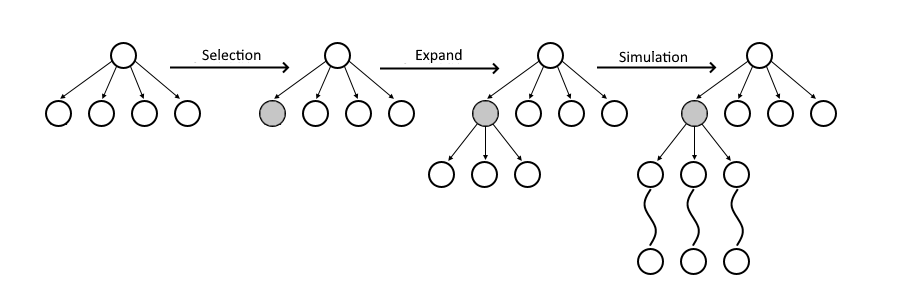
\includegraphics[width=1.0\textwidth]{pics/SelectionExpandSimulation.png}	
\caption{Auswahl eines Knotens mit nachfolgender Expansion und Simulation, eigene Abbildung}
	\label{fig:mcts_exp_sim}
\end{figure}

\begin{figure}
\centering
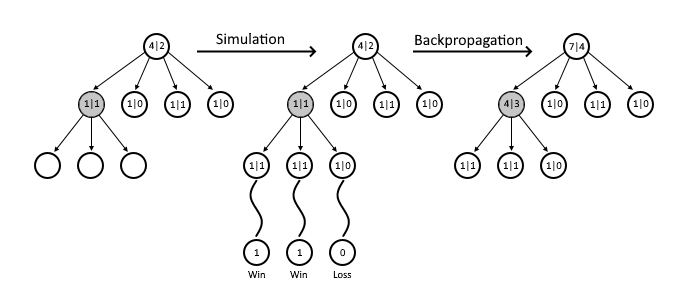
\includegraphics[width=1.0\textwidth]{pics/Backpropagation.png}
\caption{Simulation und anschließende Backpropagation der entsprechenden Werte, eigene Abbildung}
	\label{fig:mcts_backpropagation}
\end{figure}

Anzumerken ist, dass zwei verschiedene Policies genutzt werden. Für die Erweiterung des Baums wird eine Tree Policy angewendet, die besagt, dass entsprechende Blattknoten an bereits vorhandene, unbesuchte Knoten angefügt werden. Des Weiteren legt die Default Policy die Simulation fest. Hierbei wird in einem nichtterminalen Spielzustand, der gewöhnlich dem neu hinzugefügt Blattknoten entspricht, ein zufälliges Spiel durchlaufen, um ein Spielergebnis zu ermitteln \cite{Browne2012}. 

Der MCTS bleibt so lange aktiv, bis er unterbrochen wird, beispielsweise aufgrund von abgelaufener Rechenzeit. Der zu diesem Zeitpunkt als am erfolgreichsten ermittelten Knoten beziehungsweise Spielzug steht daraufhin fest \cite{Browne2012}.

Zu einem Knoten gehören der entsprechende Spielzustand, den er widerspiegelt, der Spielzug, aus dem er resultierte, sowie der aus Simulationen resultierende Reward und wie oft er besucht wurde \cite{Browne2012}.

Nachfolgend werden die konkreten Umsetzungsdetails des MCTS in AlphaGo Zero betrachtet, so wie sie von Silver et al. angewendet wurden \cite{Silver2017}.

In AlphaGo Zero wird eine Variante des Upper Confidence Bound (UCB) zur Auswahl der Knoten angewendet. Die konkrete Abwandlung ist der polynomiale UCB applied to Trees (UCT). Dieser errechnet sie wie folgt:

\begin{equation}
UCT = \frac{Q(n_i)}{N(n_i)} cP(n) \frac{\sqrt{N(n)}}{1+N(n_i)}
\end{equation} 
Wobei c eine Konstante darstellt, die das Maß an Exploration festlegt und P(s,a) für die a-priori-Wahrscheinlichkeit für die Auswahl des jeweiligen Spielzugs steht. Letztlich wird stets der Spielzug ausgewählt, der den maximalen UCT-Wert darstellt \cite{Silver2017}.
Für Abbildung \ref{fig:mcts_exp_sim} bedeutet das, dass dies im \glqq{Selection}\grqq{}-Schritt der grau hinterlegte Knoten wäre.

Ferner ist an dieser Stelle anzumerken, dass der UCB den Kompromiss zwischen Exploration und Exploitation widerspiegelt. Der erste Quotient der UCT-Gleichung steht für das Maß der Ausbeutung und lenkt den Algorithmus dahingehend vielversprechende Knoten weiter zu besuchen. Im Gegensatz dazu wird dazu angehalten Bereiche, die noch nicht oft aufgesucht wurden, verstärkt zu untersuchen. Dies wird als Erkundung bezeichnet und durch den letzten Term des UCT abgebildet. Wichtig hierbei ist es ein Gleichgewicht der beiden Komponenten zu finden \cite{Browne2012}.

Die klassische Simulation von zufälligen Spieldurchläufen entfällt im MCTS vollständig, da noch nicht expandierte Knoten an das NN weitergegeben und dort evaluiert wird. Sobald ein solcher Blattknoten erreicht ist, wird dieser dem NN übergeben, woraufhin die A-priori-Wahrscheinlichkeit und die Bewertung des Spielzugs ermittelt werden. Daraufhin ist der Blattknoten expandiert und alle ausgehenden Kanten beziehungsweise Kinderknoten werden mit initialen Werten belegt.
Anschließend erfolgt die Backpropagation, indem in allen durchlaufenen Knoten die Gewinnwahrscheinlichkeit aktualisiert, sowie die Anzahl der Besuche um den Wert Eins inkrementiert wird \cite{Silver2017}. Im Vergleich zu Abbildung \ref{fig:mcts_backpropagation} bedeutet das, dass zur Expansion des jeweiligen Knotens nicht wie bei der Simulation weiter in die Tiefe gegangen wird, um letztendlich die Endwerte \glqq{}1\grqq - \glqq{}1\grqq - \glqq{}0\grqq zu ermitteln, sondern die vom NN berechneten Werte zur Verfügung stehen. Die Backpropagation bleibt hierbei gleich.

Insgesamt wird die Baumsuche 800 mal durchlaufen\cite{SilverHubert2017}. Letztlich wird ein konkreter Spielzug ausgehend vom Wurzelknoten selektiert. Dabei wird der Knoten, der am häufigsten besucht wurde als der beste Spielzug aufgefasst. Der ausgewählte Kindknoten wird der neue Wurzelknoten. Der von ihm ausgehend aufgebaute Teilbaum wird beibehalten, während der restliche Baum verworfen wird \cite{Silver2017}.

Ferner ist anzumerken, dass Alpha(Go)Zero Kenntnis über die Spielregeln hat, die im MCTS abgerufen werden, um Spielzustände abzubilden, die aus Zügen resultieren und um Endzustände bewerten zu können \cite{Silver2017} \cite{SilverHubert2017}. 

\newpage
\subsection{Neuronales Netz}

Dieses Kapitel widmet sich zunächst der grundlegenden Funktionsweise neuronaler Netze (NN) und beinhaltet Erläuterungen zu elementaren Komponenten. Außerdem folgt eine Darlegung des spezifischen Aufbaus und der Besonderheiten des in Alpha(Go)Zero angewendeten Netzes.

\subsubsection{Grundlagen neuronaler Netze}
Ein NN wird durch eine Vielzahl einzelner miteinander verknüpfter Neuronen beschrieben. Dabei erhalten sie Signale von anderen Neuronen als Input, verarbeiten diese und geben sie als Output an andere weiter. Diese Eingangswerte werden als Vektor X = $\{x_{1}, x_{2}, ..., x_{n}\}$ repräsentiert. Um adäquate Ausgangswerte zu erhalten werden die einzelnen Input-Elemente durch die entsprechenden Komponenten im Vektor W = $\{w_{1}, w_{2}, ..., w_{n}\}$ gewichtet. Des Weiteren kann es zu jedem Neuron einen Bias b geben. Zur Verarbeitung der Eingangswerte wird eine Aktivierungsfunktion herangezogen, die Z = $\{w_{1}x_{1}, w_{2}x_{2}, ..., w_{n}x_{n} + b(W^{T}X + b)\}$ als Input erhält. Das sich hieraus ergebende Resultat entspricht \^{y}. Im weiteren Verlauf wird versucht die Diskrepanz zwischen dem tatsächlichen Wert y und dem geschätzten Wert \^{y} durch Anwendung einer Verlustfunktion zu minimieren. Dieser Vorgang wird als \glqq{}Backpropagation\grqq bezeichnet. Dabei werden Fehler von dem letzten bis hin zum ersten layer zurückgeleitet, um alle beteiligten Gewichte in die entsprechende Richtung anzupassen. Dies wird dadurch erreicht, dass man das Minimum der Fehlerfunktion lokalisiert, das durch Annäherung an den Gradienten der Funktion ermittelt werden kann \cite[S. 75-79]{Sewak2019}. 
%TODO allgemein: mathemat. Funktion, die man approximiert

Neuronale Netze bestehen aus verschiedenen Schichten. Dabei existieren stets der input layer, ein oder mehrere hidden layer und der output layer. Während der input layer über genauso viele Neuronen, wie es Eingangswerte gibt, verfügt, weist der output layer so viele Neuronen auf, wie Ausgangsmerkmale vorhanden sind. Die Neuronenzahl in den versteckten Zwischenschichten kann variieren. Sobald mehr als ein hidden layer vorliegt, spricht man von einem tiefen neuronalen Netz \cite[S. 77]{Sewak2019}. Der Aufbau wird in Abbildung \ref{fig:aufbau_nn} veranschaulicht.

\begin{figure}
\centering
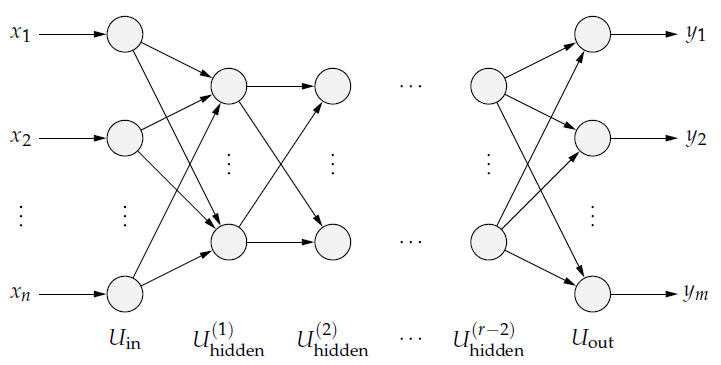
\includegraphics[width=0.6\textwidth]{pics/Aufbau_NN.png}	
\caption{Exemplarischer Aufbau eines neuronalen Netzes, Abbildung entnommen aus \cite[S. 44]{Kruse2015}}
\label{fig:aufbau_nn}
\end{figure}

Wenn in einer Schicht alle Neuronen mit allen Elementen aus dem vorangegangen sowie dem nachfolgenden layer verknüpft sind, wird diese als fully connected bezeichnet \cite[S. 79]{Sewak2019}.

Convolutional Neuronal Networks (CNNs) beschreiben tiefe Netze, die für die Bildverarbeitung ausgelegt sind. Dabei wird die Grafik typischerweise dreidimensional dargestellt, mit der Bildhöhe und -breite sowie den Farbkanälen in der Tiefe. Hierbei kann eine Schicht als convolutional layer eingebunden werden, die entsprechend eine Faltungsoperation anhand eines vorgegebenen Kerns auf das vorliegende Bild anwendet \cite[S. 85]{Sewak2019}.

Hinsichtlich der Fehlerfunktion spricht man von einem \glqq{}L1 loss\grqq{} beziehungsweise einem \glqq{}L2 loss\grqq{}, wenn der absolute respektive der quadratische Fehler berücksichtigt wird \cite[S. 82]{Sewak2019}. An dieser Stelle ist zu beachten, dass man aufgrund von möglichen negativen Differenzen nicht schlichtweg eine Aufsummierung der Fehler vornehmen kann, da sich Zahlen kleiner und größer Null sonst gegenseitig aufheben können. Deshalb muss mindestens der Betrag der absoluten Zahl genutzt werden. Meist verwendet man jedoch die quadratischen Werte, da diese Vorteile gegenüber dem Betrag aufweisen. Zunächst sind die quadratischen Werte stetig differenzierbar, wodurch die Ableitung der Fehlerfunktion vereinfacht wird. Außerdem vorteilhaft ist, dass durch die Quadrierung größere Diskrepanzen stärker gewichtet werden \cite[S. 41]{Kruse2015}.


Beispiele für Verlustfunktionen sind der \textit{mean squared error} (MSE) oder die \textit{cross entropy}.
Der MSE ist definiert durch \cite[S. 101]{Goodfellow2015}: 

\begin{equation}
f(x) = \frac{1}{m} \sum_{i} ( \hat{y}^{(test)} - y^{(test)} ) ^{2}_{i}
\end{equation}

Die Kreuzentropie wird durch folgende Funktion beschrieben \cite[S. 166]{Goodfellow2015}:

\begin{equation}
L(f_\theta (x), y) = -y log f_\theta (x) - (1 - y) log(1 - f_\theta(x))
\end{equation}

Um die Parameter eines NN zu trainieren, wird das Gradientenabstiegsverfahren genutzt. Da der Output des NN und der gewünschte Wert voneinander abweichen, wie es in der Fehlerfunktion berechnet wird, ist es das Ziel aus dieser Verlustfunktion die Richtung abzuleiten, in die die Parameter angepasst werden müssen, um die Differenz zu minimieren. Die Richtung kann festgestellt werden, indem der Gradient $ \nabla $ der Verlustfunktion ermittelt wird. Dieser stellt einen Vektor da, der die partiellen Ableitungen, also die Ableitungen nach unterschiedlichen Funktionsargumenten, der Fehlerfunktion enthält. Der Gradient dient dabei zur Repräsentation des Steigungsverhaltens einer Funktion und zeigt stets in die Richtung des höchsten Anstiegs. Um Fehler zu verringern, werden Gewichte entsprechend in die entgegengesetzte Richtung verändert. Zur Reduktion der Abweichung werden nun Fehler und Gradient berechnet, woraufhin die Anpassung der Gewichte, die Backpropagation, folgt. Zur Fehlerminimierung wird dieser Prozess iterativ durchlaufen. Zur Berechnung des Fehlers des gesamten NN werden die jeweiligen einzelnen Diskrepanzen aufaddiert \cite[S. 58-60]{Kruse2015}. Ein ein ausführliches Beispiel zur Fehlerminimierung und Berechnung der partiellen Ableitungen findet sich in \cite[S. 64-68]{Kruse2015}.
Des Weiteren ist zu berücksichtigen, dass beim Gradientenabstieg grundsätzlich nicht gewährleistet werden kann, dass ein globales Minimum gefunden wird. Lediglich die Annäherung an ein lokales Minimum kann sichergestellt werden \cite[S. 69]{Kruse2015}. Ein weiteres Problem beim vorgestellten Verfahren ist, die Wahl der optimalen Lernrate $ \theta $, die die Schrittweite angibt. Das bedeutet, je kleiner die die Lernrate ist, desto langsamer, in kleineren Schritten, approximiert man das gesuchte Minimum. Dies kann unter Umständen zu viel Zeit in Anspruch nehmen. Wählt man für die Lernrate allerdings einen großen Wert, so nähert man sich dem gewünschten Punkt in entsprechenden großen Schritten an. Auf diese Weise kann es passieren, dass das Minimum stets übersprungen wird \cite[S. 67]{Kruse2015}. 
%TODO Grafik: Man erkennt diesen Prozess...
%TODO optimale Werte für theta

Eine Möglichkeit diesem Problem bei einer gleichzeitig hohen Lernrate entgegenzuwirken liegt in der Inklusion des Momentums. Dabei wird der Wert der vorangegangenen Richtung für die Berechnung der neuen Richtung berücksichtigt, wodurch Oszillationen verringert werden und das Minimum schneller erreicht wird \cite{Rumelhart1985}.

Als Hyperparameter bezeichnet man in NN Konfigurationsparameter, durch die man das Verhalten des Netzes steuern kann. Diese Variablen werden manuell festgelegt und nicht wie die übrigen Netz-Parameter vom Programm gelernt \cite[S. 113]{Goodfellow2015}.
%TODO Aktivierungsfunktion grafiken, tanh, relu, 
Laut Nwankpa, Ijomah, Gachagan \& Marshall beeinflussen sowohl Hyperparameter als auch Aktivierungsfunktionen die Generalisierbarkeit sowie die Effektivität des Lernprozesses \cite{Nwankpa2018}. Dementsprechend wichtig ist es eine Aktivierungsfunktion auszuwählen, die möglichst gut für den spezifischen Anwendungsfall geeignet ist. Mithilfe von AF wird entschieden, ob ein Neuron gefeuert wird oder nicht. Der Output eines NN berechnet sich durch y = $(w_{1}x_{1}, w_{2}x_{2}, ..., w_{n}x_{n} + b)$, was grundsätzlich einem linearen Ergebnis entspricht. Für den Lernprozess werden jedoch nicht-lineare Daten benötigt, da diese differenzierbar sind. Daher bilden AF die Ausgabedaten eines NN innerhalb eines bestimmten Wertebereichs ab und wandeln sie in nicht-lineare Werte um. Daher ergibt sich, y = $ \alpha (w_{1}x_{1}, w_{2}x_{2}, ..., w_{n}x_{n} + b)$ für den Output, wobei $\alpha $ für die entsprechende AF steht \cite{Nwankpa2018}.

Ein Beispiel für eine Aktivierungsfunktion ist der tangens hyperbolicus (tanh), der durch 
\begin{equation}
f(x) = \frac{e^x - e^{-x}}{e^x + e^{-x}}
\end{equation}
repräsentiert wird \cite{Nwankpa2018} und dessen grafischer Verlauf in Abbildung \ref{fig:tanh} ersichtlich wird. Die Funktionen bildet Eingaben auf einen Wertebereich zwischen -1 und 1 ab. Ihre Stärke ist, dass sie null-zentriert ist, ihre Schwäche hingegen, dass mit ihr weiterhin verschwindende Gradienten vorkommen können \cite{Nwankpa2018}.

\begin{figure}
\centering
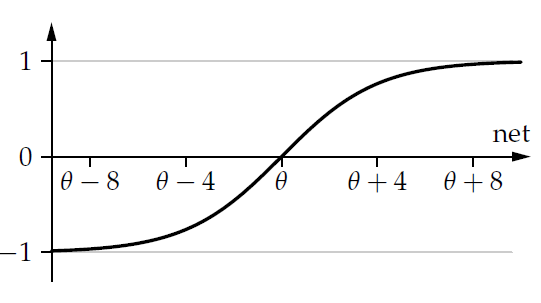
\includegraphics[width=0.4\textwidth]{pics/tanh.png}	
\caption{Grafischer Verlauf der tanh-Funktion, Abbildung entnommen aus \cite[S. 45]{Kruse2015}}
\label{fig:tanh}
\end{figure}

Die rectified linear unit (ReLU) bietet ebenfalls die Möglichkeit zur Aktivierung der Neuronen und ist gegeben durch:


\begin{equation}
 f(x) = max (0, x) = 
\begin{cases}
      x_i, & \text{if $x_i \geq 0$}\\
      0, & \text{if $x_i<0$}
    \end{cases}
\end{equation}

Negative Eingabewerte werden hierbei auf den Null abgebildet, wodurch vanishing gradients vermieden werden können. Allerdings ist der gravierendste Nachteil dieser Funktion, dass sie zu sogenannten dead neurons führen kann \cite{Nwankpa2018}. 
Hinsichtlich dieses Problems kann jedoch die leaky ReLU (LReLU) Abhilfe schaffen, die die durch folgende Formel beschrieben wird:

\begin{equation}
 f(x) = \alpha x + x = 
\begin{cases}
      x, & \text{if $x > 0$}\\
      \alpha x, & \text{if $x \leq $}
    \end{cases}
\end{equation}

Durch die Multiplikation der Konstante $\alpha$, die den Wert 0.01 annimmt, können die Gradienten während des Trainings niemals Null werden \cite{Nwankpa2018}.

Für eine detaillierte Analyse bestehender Aktivierungsfunktionen sei auf Nwankpa et al. \cite{Nwankpa2018} verwiesen.

Ein weiteres Problem, bei dem Aktivierungsfunktionen Hilfestellung leisten ist das des vanishing beziehungsweise exploding gradient. Durch die wiederholte Multiplikation der Ableitungsterme, die entweder kleiner oder größer Eins sind, werden die Ergebnisse im Laufe der Zeit teils entweder verschwindend gering oder unendlich groß. AF können diese Werte durch entsprechende Abbildung innerhalb eines bestimmten Rahmens halten und dem Problem somit entgegenwirken \cite{Nwankpa2018}.

Ein weiteres wichtiges Hilfsmittel findet sich in der Batch Normalisation, mithilfe der Mittelwerte und Varianzen in den Eingabedaten der einzelnen Schichten normalisiert werden können. Das ist sinnvoll, da sich die Schichten sonst laufend an die neue Verteilung anpassen müssen. Der ausschlaggebende Vorteil der Normalisierung ist, dass das Modell deutlich effizienter trainiert werden kann, da höhere Lernraten angewendet werden können  \cite{Ioffe2015}.

Tiefe NN sind schwer zu trainieren. Zur Vereinfachung dieser Problematik besteht die Möglichkeit Abkürzungen zu nutzen. Die Vorgehensweise wird in Abbildung \ref{fig:res_skip} deutlich. Dabei können Daten (siehe \glqq{}x\grqq) bestimmte Schichten (vergleiche \glqq{}weight layer\grqq) überspringen und werden somit in diesen layern nicht verarbeitet, sondern gehen direkt weiter zu einem vorgegebenen Punkt im NN. Diese Methode wird \glqq{}residual learning\grqq{} genannt und optimiert den Umgang mit tiefen Netzen \cite{He2016}.

\begin{figure}
\centering
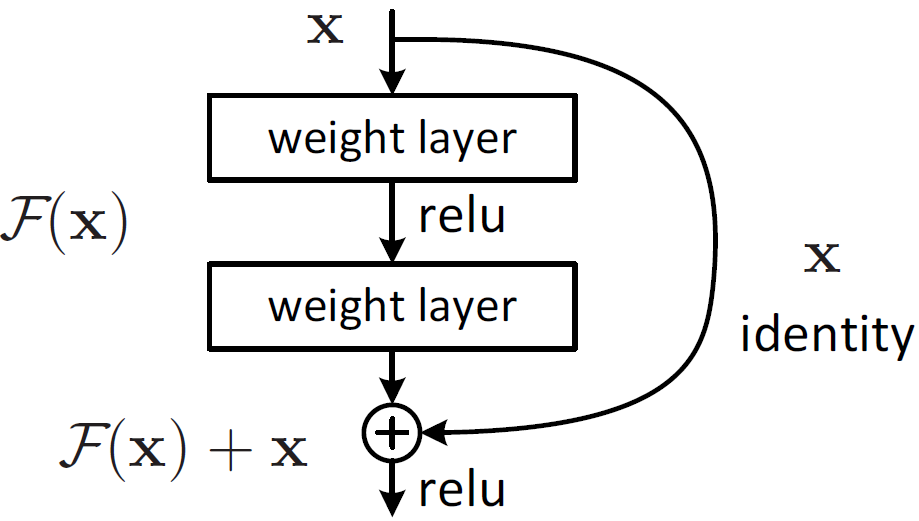
\includegraphics[width=0.4\textwidth]{pics/res_skip_connection.png}	
\caption{Darstellung einer möglichen Abkürzung in residual nets, Abbildung entnommen aus \cite{He2016}}
\label{fig:res_skip}
\end{figure}

Für detaillierte Erläuterungen zu NN wird auf das Grundlagenwerk \cite{Goodfellow2015} verwiesen.

\subsubsection{Neuronales Netz in Alpha(Go)Zero}
\label{secNNAZ}
Der Input für das NN in AlphaZero besteht aus mehreren Ebenen, die die Größe des Spielfeldes annehmen. Für jeden Spielzustand existiert eine Kombination aus mehreren Ebenen, die diesen exakt abbilden. Dabei gibt es für jeden Input-Typ, beispielsweise Spielsteine von Spieler 1 oder von Spieler 2, eine solche Fläche, die durch binäre Codierung angibt, ob die entsprechende Eingabe auf der jeweiligen Position vorhanden ist oder nicht \cite{SilverHubert2017}.

Das in AlphaGo Zero und AlphaZero verwendete NN zeigt nachfolgenden von \cite{Silver2017} beschriebenen Aufbau.
Zunächst werden die Eingabedaten in einem \textit{residual block} verarbeitet. Dieser besteht aus einem \textit{convolutional block} und nachfolgend 19 oder 39 residualen Blöcken. Erst genannter führt eine Faltungsoperation mit 256 Filtern mit einem 3x3 Faltungskern und einer Schrittweite von 1 durch. Anschließend folgt die \textit{Batch Normalisation} sowie die Aktivierung mithilfe der ReLU. Die Restblöcke verfügen ebenfalls über die drei genannten Komponenten – Faltung, Normalisierung und Aktivierung sowie zusätzlich darauf anschließend erneut eine Faltung mit den gleichen Eigenschaften, gefolgt von der \textit{Batch Normalisation} und der Endposition der Abkürzungsmöglichkeit der Eingabedaten. Abschließend findet sich erneut die ReLU.
Die resultierenden Daten werden an den den sogenannten \glqq{}Policy Head\grqq{} sowie den \glqq{}Value Head\grqq{} weitergereicht. Diese beiden Komponenten sind für das Berechnen der \textit{Policy} beziehungsweise der Spielbewertung zuständig. Der \textit{Policy Head} setzt sich aus einer Faltung mit zwei Filtern mit einem 1x1 Faltungskern und einer Schrittweite von 1, einer Normalisierung, der ReLU und einem \textit{fully connected layer} zusammen. Letzterer gibt einen Vektor zurück, der die Logit-Wahrscheinlichkeiten für alle realisierbaren Aktionen beinhaltet.
Die ersten drei Schritte sind gleichermaßen im \textit{Value Head} wiederzufinden. Allerdings folgt hier ein \textit{fully connected layer} mit einer versteckten Schicht. Des Weiteren durchlaufen die Daten die ReLU und erneut eine vollständig verknüpfte Schicht, die in einem Skalar resultiert. Dieser wird abschließend durch die Aktivierungsfunktion tanh auf einen Punkt im Wertebereich zwischen [-1, 1] abgebildet \cite{Silver2017}.

Letztendlich beschränkt sich die der Output des NN auf zwei Komponenten, nämlich dem policy und dem value head. Der policy head gibt für jede Position im Spielfeld eine A-priori-Wahrscheinlichkeit zurück, die angibt mit wie wahrscheinlich es ist, dass der Spieler seinen Spielstein auf dieses Feld legt. Der value head hingegen bewertet den Spielzustand und gibt an, wie wahrscheinlich es ist, dass der Spieler in diesem Zustand gewinnt \cite{Silver2017}.

Trainiert wird das NN durch Spiele gegen sich selbst. In AlphaGo Zero gibt es dabei zwei Instanzen. Das neu trainierte Modell wird nach jedem Trainingsdurchlauf mit dem derzeit besten Modell verglichen. Falls das neue Modell in 55 \% der Spiele gegen das beste gewinnt, so wird das beste Modell überschrieben. In beiden Varianten werden die Parameter zunächst zufällig initialisiert. Für AlphaZero gibt es aber lediglich eine Instanz, deren Parameter laufend aktualisiert werden \cite{SilverHubert2017}. 

\subsection{Reinforcement Learning}
Reinforcement Learning (RL), auch als bestärkendes Lernen bezeichnet, beschreibt die Interaktion eines Agenten mit einer konkreten Environment. Dabei stellt die Umgebung dem Agenten einen bestimmten Zustand bereit, anhand dessen er die bestmögliche Aktion auswählt, die im nächsten Schritt ausgeführt werden soll. Daraufhin wird der Zustand entsprechend modifiziert und eine Funktion berechnet, die dem Agenten eine Belohnung oder Bestrafung in Form eines positiven beziehungsweise negativen Rewards zurückliefert. Anhand iterativer Durchläufe von Lern- und Entscheidungsprozessen optimiert der Agent seine Aktionen. Dies ist in Abbildung \ref{fig:rl_agent_loop} einzusehen. Dabei wählt der Agent zunächst Aktion $a_{t}$ im Zustand $s_{t}$, was eine Änderung des Zustands der Umgebung zu $s_{t+1}$ zur Folge hat. Außerdem berechnet die Environment den Reward $r_{t}$ für die vom Agenten gewählte Aktion. Ziel in diesem Trainingsdurchlauf für den Agenten ist es, anhand der Belohnungsstrategie die Entscheidung bezüglich der besten nächsten Aktion zu stetig zu verbessern. Hierbei anzumerken ist, dass die Rewardfunktion sowohl den Zustand als auch die Aktion berücksichtigt, um einen Rückgabewert zu berechnen. Daraus folgt, dass die gleiche Aktion unterschiedlichen Ausgangszuständen in verschiedenen Belohnungswerten resultieren kann beziehungsweise sogar sollte \cite[S. 2]{Sewak2019}.

Die Strategie zur Ermittlung der besten Aktion während des Lernprozesses wird als Policy $\pi$ bezeichnet. Diese ist während eines gesamten Trainingsdurchlaufs gültig. Bezüglich der Notation gibt $\pi_{(s)}$ entsprechend die vielversprechendste Aktion im Zustand s an \cite[S. 16]{Sewak2019}.

\begin{figure}
\centering
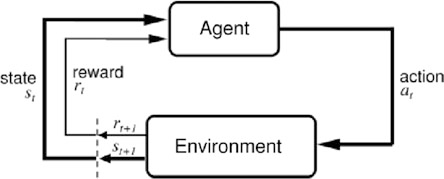
\includegraphics{pics/rl_agent_loop.png}	\caption{iterative Interaktion zwischen Agent und Environment, Abbildung entnommen aus \cite[S. 2]{Sewak2019}}
\label{fig:rl_agent_loop}
\end{figure}

Ferner bringt das Aufstellen einer Rewardfunktion Schwierigkeiten mit sich, da sie versucht eine sinnvolle Vorhersage für die Bewertungen eines Zustandes zu ermitteln. Probleme können dabei beispielsweise darin liegen, dass Belohnungen womöglich erst im zukünftigen Verlauf zu Tage treten können oder dass sie zum gegenwärtigen Zeitpunkt schlichtweg noch ungewiss sind. Mögliche Lösungen hierfür sehen allerdings je nach Anwendungsdomäne verschieden aus \cite[S. 4-7]{Sewak2019}.

Reinforcement Learning Modelle sind als \glqq{}Markov Devision Process\grqq{} (MDP) anzusehen. Das hat zur Folge, dass aufgrund der zugrundeliegenden \glqq{}Markov Property\grqq{} sowie \glqq{}Markov Chain\grqq{} die Wahrscheinlichkeiten für die nächstmöglichen Aktionen lediglich vom derzeitigen Zustand und nicht von weiteren vorangegangen abhängen. Der MDP wendet diese Regeln auf den Entscheidungsprozess an, der im Fall von RL die Policy darstellt. Des Weiteren liefert der MDP die Wahrscheinlichkeiten für Zustandsübergange in der Form $P_{a}(s, s')$ an, wobei a für die mögliche Aktion, s für den aktuellen und s' für den resultierenden Zustand steht. Die Notation des entsprechenden Rewards lautet $R_{a}(s, s')$ \cite[S. 19f.]{Sewak2019}.

Weitere Begriffe, die im Kontext von RL von Bedeutung sind, sind \glqq{}Policy Evaluation\grqq{} und \glqq{}Policy Iteration\grqq{}. Erstere steht für die geschätzte Bewertung des Zustandes. Letztere beschreibt einen Iteration Prozess mit dem Ziel, dass die Policy konvergiert \cite[S. 27]{Sewak2019}.

\subsection{Zusammenspiel von Monte Carlo Tree Search und neuronalem Netz}
AlphaGoZero und AlphaZero basieren auf der Kombination des MCTS und des NN. Dabei gibt es zwei Schnittstellen zwischen diesen beiden Komponenten. 
Erstere liegt in der bereits erwähnten Bewertung von Blattknoten. Der MCTS durchläuft keinen simulierten Spielablauf, sondern überlässt die Evaluation des Knotens dem NN und arbeitet mit den zurückgegebenen Daten weiter. Dies spiegelt die policy evaluation wider \cite{Silver2017}.

Eine weitere Verzweigung von MCTS und NN tritt bei dem Update der Parameter des NN auf. Das NN ermittelt zu jedem Spielstand die möglichen Züge und gibt deren Gewinnwahrscheinlichkeit sowie die Wahrscheinlichkeit für die Auswahl des Zuges an. Für die Aktualisierung der Parameter werden die genannten Werte dahingehend angepasst, dass sie den im MCTS ermittelten Werten entsprechend beziehungsweise sich diesen annähern. Eine Anpassung in diese Richtung ist sinnvoll, da die Daten im MCTS als deutlich genauer gelten. Dieser Vorgang entspricht der policy improvement \cite{Silver2017}.

\newpage
% ----------------------------------------------------------------------------------
% Kapitel: Implementierung/Umsetzung
% ----------------------------------------------------------------------------------
\section{Implementierung}

\subsection{Aufbau des Programms}
Der Aufbau des Programms unterteilt sich fünf größere Bereiche: \texttt{General}, \texttt{Server Communication}, \texttt{Environment}, \texttt{Monte Carlo Tree Search} und \texttt{Neuronales Netz}. In folgenden Abschnitten werden alle Bereiche kurz erläutert und deren Funktionsweise geschildert.

\subsubsection{General}
Das Paket \texttt{General} beinhaltet die Grundfunktionalität des Programms sowie verbindende Elemente zwischen mehreren Paketen.
So befindet sich hierin unter anderem die \texttt{Main}-Klasse mit der das Programm gestartet wird, mitsamt der zugehörigen Grundfunktionalität. Hier wird der Standardablauf des Spielstarts und eines Spielzuges definiert sowie die weiteren benötigten Klassen initialisiert. Des Weiteren k\"{u}mmert sich die Klasse um die Nutzung der Grafikkarte (ob mehrere Grafikkarten genutzt werden d\"{u}rfen) und um den Aufbau des Trainings des Neuronalen Netzes am Spielende.\\
Des Weiteren beinhaltet das Paket die Definition der Kommandozeilenparameter sowie spielrelevante und klassenübergreifende Konstanten.

\subsubsection{Server Communication}
In diesem Bereich wird die Kommunikation zwischen Programm und Server abgebildet. Es wird eine Verbindung zum Server aufgebaut und auf jede Nachricht reagiert. Eine vollständige Spezifikation darüber, welche Nachrichten der Server versendet, ist in der Spezifikation des Wahlpflichtfachs: Client-K.I.s für Brettspiele (ReversiXT) zu finden.

Die Initialisierungsphase besteht aus der Registrierung unseres Programms am Server, der Zuweisung der zugehörigen Spieler-Nummer und des Aufbaus des Spielfelds. Hier wird zunächst eine Verbindung zum Server aufgebaut und dieser vergibt die Spieler-Nummer. Sobald alle Spieler eines Spielfelds registriert sind, beginnt der Server das Spielfeld zu versenden. Das Spielfeld besteht aus einem String, der an die Funktion \texttt{parseRawMap} im Bereich \texttt{Environment} weitergegeben wird. Nachdem das Spielfeld eingelesen ist, wird auf weitere Anweisungen des Servers gewartet. Zu diesem Zeitpunkt kommen Anweisungen in Form einer Zugaufforderung oder es wird ein Spielzug eines Gegners geschickt. In beiden Fällen wird das \texttt{Environment} benachrichtigt diese Anweisung auszuführen. Wenn der Server eine Disqualifizierung oder ein Spielende verschickt, wird das Programm beendet.

\subsubsection{Environment}
Zum Bereich \texttt{Environment} gehören die Klassen \texttt{Environment}, \texttt{Player}, \texttt{Playground} und \texttt{Turn}. Hauptsächlich sind hier Funktionen vorhanden, die zum Spielen benötigt werden.

\begin{itemize}

\item{Jeder Spieler wird als eine eigene Instanz der Klasse \texttt{Player} angelegt. In der Klasse wird das Spieler-Symbol gespeichert. Alle weiteren Funktionen der Klasse haben in unserer Version des Programms keine Auswirkung.}

\item{Die Klasse \texttt{Turn} wird verwendet, um Spielzüge darzustellen, daher sind Variablen für die Position des Spielzugs und das Spieler-Symbol vorhanden. Die Variable mit dem Namen \texttt{prior} wird für die Bewertung eines Zuges verwendet. Wie hoch diese Bewertung ist entscheidet das Neuronale Netz und die Verwendung wird in Abschnitt \ref{MCTS} beschrieben. Es wird zusätzlich noch gespeichert welcher Wert auf dem Spielbrett an der Position des Spielzugs steht.}

\item{In der Klasse \texttt{Playground} wird das Spielfeld sowie die zugehörige Höhe und Breite abgespeichert. Die Funktion \texttt{updatePlaygroundPhase1} führt einen Zug auf das Spielfeld aus, welches in der Klasse selbst gespeichert wird. Hierzu wird ein \texttt{Turn} und ein \texttt{Player} übergeben. Damit anhand der Spielregeln geprüft werden kann, ob ein Zug gültig ist, wird die Funktion \texttt{validateTurnPhase1} verwendet. Dieser Funktion werden ebenso \texttt{Turn} und \texttt{Player} übergeben, der Rückgabewert gibt an, ob der Zug gespielt werden darf. Innerhalb des Programms ist es oft notwendig ein Spielfeld zu kopieren, dafür wird die Funktion \texttt{getCloneOfPlayground} verwendet.}

\item{Die Klasse \texttt{Environment} wird während der Programmausführung nur einmal global instantiiert. Hier wird immer das derzeitige Spielfeld gespeichert und nach jedem Spielzug, der zum Server geschickt oder empfangen wird, aktualisiert. Weiterhin wird ein Array aller \texttt{Player}-Instanzen und eine Referenz auf unsere \texttt{Player} Instanz gespeichert. Um den nächsten Spieler in der Zugreihenfolge zu erhalten gibt es die Funktion \texttt{getNextPlayer}.}

\end{itemize}

\subsubsection{Monte Carlo Tree Search}
Sobald unser Programm eine Zugaufforderung vom Server erhalten ruft die \texttt{Main}-Funktion den MCTS auf. Der MCTS baut im groben einen Suchbaum auf, indem verschiedene Spielzüge simuliert werden. Mithilfe eines NN werden Spielzüge bewertet, wodurch der MCTS den am besten bewerteten Spielzug zurückgeben kann. Eine detaillierte Implementierung ist in Abschnitt \ref{MCTS} gegeben.

Für den MCTS war eine neue Klasse \texttt{Node} notwendig, die Spielzüge mit ihren zugehörigen Spielfeldern beinhaltet. Die \texttt {Nodes} repräsentieren Knoten des Suchbaums, daher ist es wichtig den vorherigen Knoten (\texttt{Node parent}) und alle nachfolgenden Knoten (\texttt{ArrayList<Node> children}) zu speichern.

\subsubsection{Neuronales Netz}
Das NN wird innerhalb des MCTS verwendet, um Spielfelder und Spielzüge zu bewerten. Hierfür wird dem NN ein Spielfeld und der Spieler, der den nächsten Zug auf diesem Spielfeld hat, übergeben. Die Rückgabe besteht aus einer Zahl zur Bewertung des Spielfeldes und einem Array mit einer Bewertung für jede Position des Spielfeldes. In der Klasse \texttt{NeuronalNet} befindet sich die Definition des Modells des neuronalen Netzes. Des Weiteren fungiert die Klasse \texttt{PolicyValuePredictor} als Wrapper über das neuronale Netz und bietet Schnittstellen für das Laden und Speichern von Modellen, für das Training und die Evaluation von Zuständen. Um den Input vom MCTS für das NN zu transformieren, wird die Klasse \texttt{PlaygroundTransformer} genutzt. 

\subsection{Monte Carlo Tree Search}\label{MCTS}
Um den MCTS für Reversi zu realisieren wurden die Klassen MCTS und Node angelegt. Letztere enhält zwei überladene Konstruktoren zum Anlegen von Wurzel- und Kindknoten. Ein Node enthält zusätzliche Attribute. Sowohl der Elternknoten als auch eine ArrayList vom Typ Node, die die direkten Kinder enthält, werden abgespeichert. Die Anzahl, wie oft ein Knoten besucht wurde, wird in der Variablen \texttt{numVisited} hinterlegt. Außerdem gespeichert wird das Ergebnis eines simulierten Spieldurchlaufs in \texttt{simulationReward}. Der aktuelle Spielzustand, der im Playground repräsentiert wird, wird ebenfalls im Node hinterlegt. Des Weiteren wird in dem Attribut \texttt{nextPlayer} festgehalten, welcher Spieler als Nächstes an der Reihe ist und welche Züge (\texttt{nextTurns}) dieser als nächstes ausspielen kann. Für das Training werden außerdem die vom NN erhaltenen A-Priori-Wahrscheinlichkeiten abgespeichert. Dies geschieht allerdings ausschließlich, wenn der dem \texttt{Node} zugehörige \texttt{Turn} vom Agent gespielt wird.

Es gibt einen überladenen Konstruktor, der einerseits für das Anlegen einer neuen Wurzel und andererseits für das Erzeugen eines neuen Kinderknotens zuständig ist. Bei der Instanziierung durch die Konstruktoren werden sinnvolle initiale Werte vergeben. \texttt{numVisited} und \texttt{simulationReward} werden auf 0 beziehungsweise 0.0  für den \texttt{root}, und 1 beziehungsweise dem vom NN erhaltenen, übergebenen \texttt{reward} gesetzt. Für den Wurzelknoten gilt, dass er keinen Parent besitzt, für alle weiteren Knoten wird der Parent übergeben und gesetzt. Die Children werden zunächst durch eine leere Liste initialisiert. Der \texttt{nextPlayer} wird ebenfalls übergeben und gesetzt. Außerdem zu erwähnen ist die Methode \texttt{calculateUCT()}, die den Upper Confidence Bound applied to Trees (UCT) für einen Knoten berechnet. Sie ermittelt zunächst die Exploitation-Komponente, indem sie den simulationReward durch die Anzahl an Besuchen dividiert. Die Exploration berechnet sich aus dem Verhältnis, wie oft der Parent besucht wurde, geteilt durch den inkrementierten Wert, wie oft der aktuelle Knoten besucht wurde. Aus dem Quotienten wird anschließend die Wurzel gezogen. Um den Kompromiss zwischen diesen beiden Komponenten zu kontrollieren, wird die Exploration mit einer festgelegten Konstante und der A-priori-Wahrscheinlichkeit, die im NN trainiert wird, für einen Zug multipliziert. Die Konstante verhält sich wie ein Hyperparameter und wurde daher manuell festgelegt. In anderen recherchierten Projekten wurden beispielsweise Werte zwischen 1 und 6 getestet, wobei sich ein Wert Nahe an 4 als ideal herausstellte \cite{MediumPart3}. Daher haben wir ebenfalls verschiedene Einstellungen getestet und konnten mit einem Wert von 3.5 das beste Ergebnis erzielen.

Da die Implementierung des MCTS vor der des NN stattfand, entstanden zwei lauffähige Versionen, sodass einerseits eine Baumsuche ohne Zusammenarbeit mit dem NN , andererseits aber mithilfe des NN durchgeführt werden kann. Da in erst genannte ebenfalls viel Aufwand investiert wurde, bleibt diese zusätzlich erhalten. Dafür spezifische Methoden wurden mit \glqq{}\texttt{\_deprecated}\grqq{} versehen.

Hinsichtlich der Klasse \texttt{MCTS} ist festzuhalten, dass diese das Interface \texttt{ITurnChoiceAlgorithm} implementiert und in der Klasse \texttt{Agent} über den Konstruktoraufruf instanziiert wird. Dieser verlangt das Environment und den Player als Übergabeparameter und legt daraufhin einen neuen Wurzelknoten an sowie eine leere \texttt{ArrayList} vom Typ \texttt{Node}, die die Blattknoten beinhaltet, die im späteren Verlauf simuliert werden müssen. Für die Simulation muss beachtet werden, dass die Environment geklont und somit eine tiefe Kopie erzeugt werden muss, damit der tatsächliche Spielzustand nicht unbeabsichtigt manipuliert wird. 

Der nächste Abschnitt widmet sich dem Code zur Baumsuche im Zusammenspiel mit dem NN, dessen Ablauf in Abbildung\footnote{Erstellt mit astah (https://astah.net/)} \ref{fig:mcts_seq} veranschaulicht wird. Zunächst wird über die öffentliche Interface-Methode \texttt{chooseTurnPhase1()} die private Methode \texttt{searchBestTurn()} aufgerufen. Hierbei wird zunächst über die globale Variable \texttt{firstCall} überprüft, ob die Baumsuche mit einem neuen Wurzelknoten startet oder ob der nächste zu evaluierende Knoten ausgewählt werden muss. Für letzteren Fall gilt, dass im \texttt{else}-Block der Knoten mit dem größten UCT-Wert ausgehend von der Wurzel ermittelt wird. Dazu wird \texttt{searchBestUCT()} aufgerufen. Falls man sich im ersten Aufruf befinden, wird \texttt{root} zur Evaluation an das NN übergeben. Dies geschieht durch den Aufruf von \texttt{evaluate(playground, player)} aus der Klasse \texttt{PolicyValuePredictor}, wobei der entsprechende Spielzustand und Spieler übergeben werden. Als Rückgabe erhält man die Zustandsbewertung (\texttt{reward}) und die A-prior-Wahrscheinlichkeiten \texttt{priors} als Array vom Typ \texttt{double}. Diese \texttt{priors} signalisieren die Wahrscheinlichkeit, dass ein der Spieler im nächsten Zug einen Spielstein auf ein bestimmtes Feld setzt. Da dabei alle Positionen im Spielfeld berücksichtigt werden, werden anschließend lediglich die gültigen Züge mithilfe der Funktion \texttt{getPossibleTurns} herausgefiltert und um ihre jeweilige A-priori-Wahrscheinlichkeit ergänzt. Da die Wurzel nun bewertet wurde, werden die nächstmöglichen Züge (\texttt{setNextTurns(validTurns)}) sowie ihre Zustandsbewertung (\texttt{setSimulationReward(reward)}) gesetzt. Außerdem wird die hinterlegte Anzahl der Besuche im \texttt{root} inkrementiert (\texttt{incNumVisited}). Abschließend wird der Wurzelknoten als \texttt{bestUCTNode} hinterlegt und \texttt{firstCall} wird auf \texttt{FALSE} gesetzt. 

Unabhängig davon, welche Ausgangssituation vorlag, wird als nächstes eine \texttt{while}-Schleife durchlaufen, die erst abbricht, wenn es keinen weiteren Folgeknoten zur Evaluation gibt (\texttt{bestUCT == null}) oder sobald 800 Simulationen (siehe Konstante \texttt{NR\_SIMULATIONS} ) durchgeführt wurden. Innerhalb der Schleife wird stets ein Knoten mithilfe der Funktion \texttt{createNextNodeAndEvaluate(bestUCTNode)} evaluiert. Diese sucht zunächst durch die Funktion \texttt{choseNextTurn} den Zug aus, der ausgehend von dem übergebenen Knoten als nächstes gemacht werden soll. Das Entscheidungskriterium hierfür liegt in der höchsten A-priori-Wahrscheinlichkeit. Anschließend wird der \texttt{playground} entsprechend dem ausgewählten Zug aktualisiert und zur Bewertung an das NN übergeben. An dieser Stelle passiert selbiges wie oben bereits für den Wurzelknoten beschrieben. Abschließend wird jedoch ein neuer Knoten für den durchgeführten \texttt{turn} erstellt, der anfangs übergebene Knoten erhält den neuen Knoten als Kind und der betrachtete Spielzug wird aus der Liste der nächstmöglichen Züge entfernt.

Nachdem die Evaluation abgeschlossen ist, wird der ermittelte Wert für den Knoten anhand der Methode \texttt{backpropagate()} zurück übermittelt. Dabei wird der \texttt{reward} des übergebenen \texttt{node} an alle in der Hierarchie über ihm stehenden Knoten übermittelt. Zusätzlich wird die Anzahl an Besuchen der entsprechenden Knoten inkrementiert. Daraufhin wird in der Methode \texttt{setBestTurn} der Zug ermittelt, der aktuell als am besten interpretiert wird. Ausschlaggebend hierfür ist, welcher Knoten am öftesten besucht wurde. Abschließend wird erneut der als nächstes zu evaluierende Knoten durch \texttt{searchBestUCT} ermittelt, wodurch die Iteration erneut beginnt.

\begin{figure}
\centering
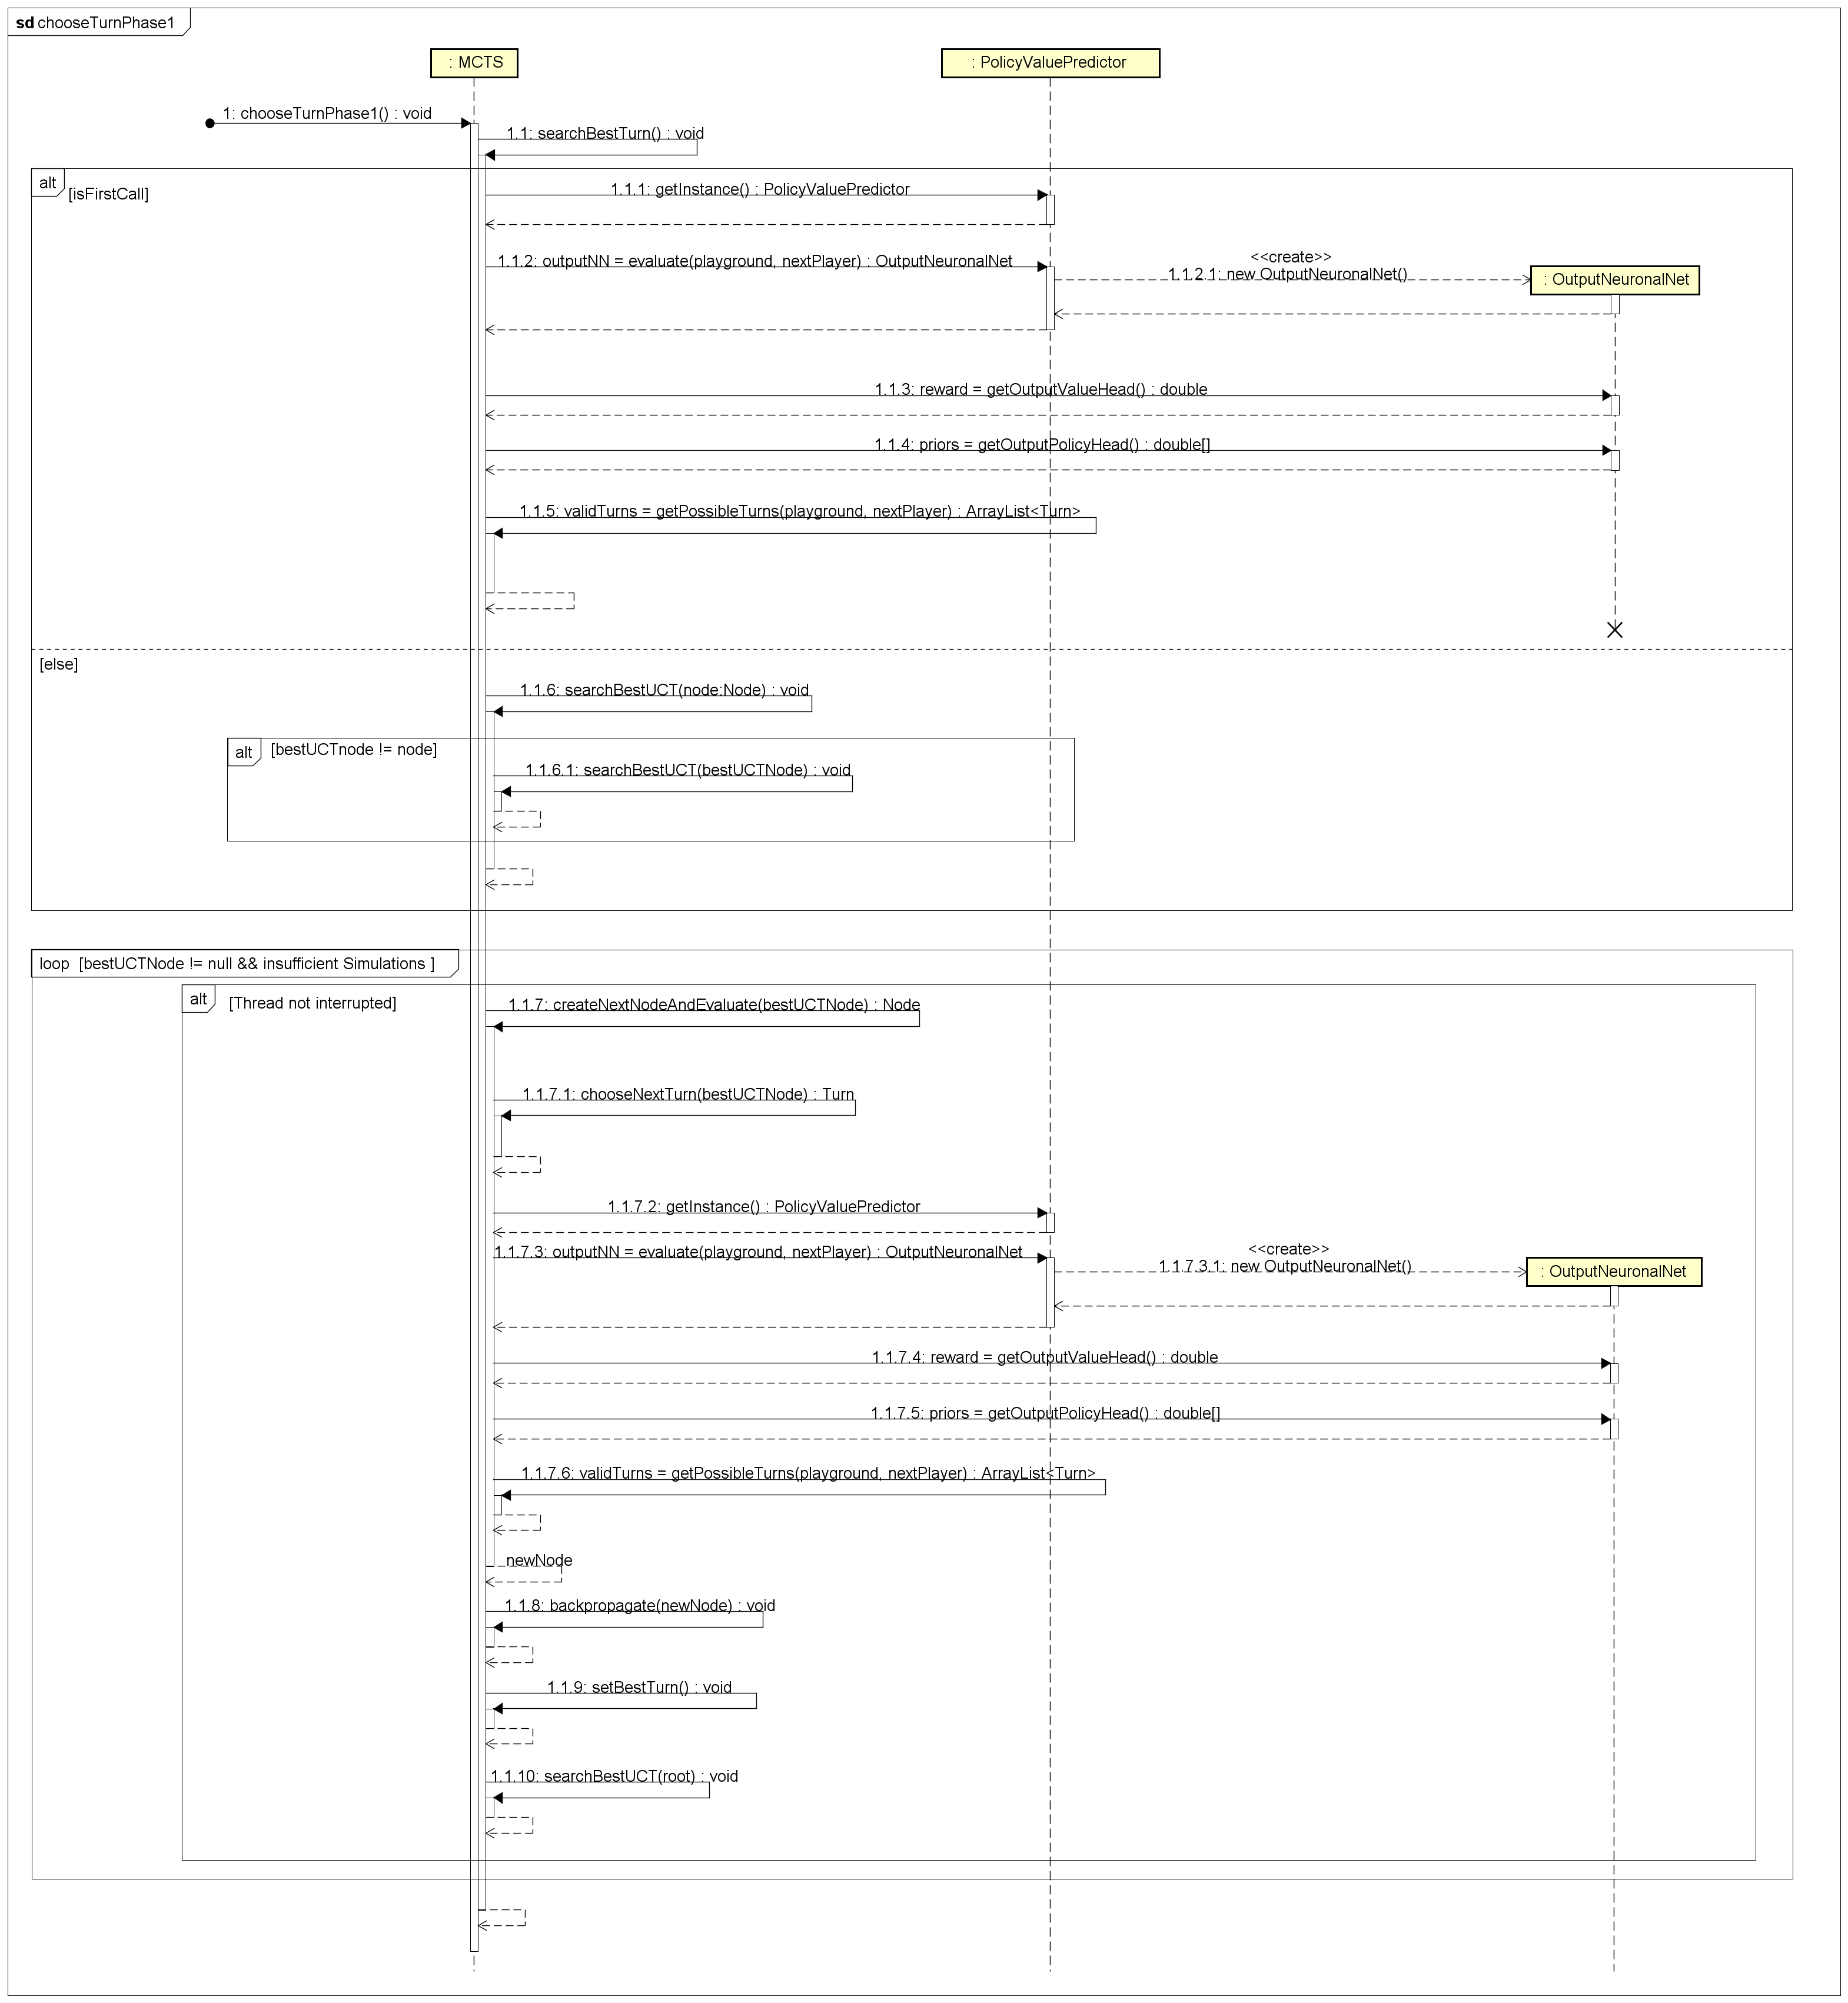
\includegraphics[width=1.0\textwidth]{pics/mcts_seq.png}	
\caption{Sequenzdiagramm der wichtigsten Komponenten des MCTS, eigene Abbildung erstellt mit astah}
\label{fig:mcts_seq}
\end{figure}

Nachfolgend wird die Implementierung für den MCTS ohne NN erläutert. Beim Klonen der Environment ist festzuhalten, dass dies zweimal stattfindet. Einmal, wenn ein neuer Baum aufgebaut wird, somit erhält der neue Wurzelknoten und ebenfalls jedes seiner Kinder jeweils einen eigenen Klon. Für die Kinderknoten gilt, dass diese ihre Environment-Instanz an ihre Kinder weitergeben und diese somit innerhalb derselben Instanz agieren. Um den MCTS zu starten, wird die Methode \texttt{searchBestTurn()} aufgerufen. Diese expandiert zunächst den Wurzelknoten, indem sie alle im aktuellen Zustand möglichen validen Züge ermittelt und durch diese iteriert. Die Methode \texttt{getPossibleTurns()} gibt diese zurück. Sie iteriert über das gesamte Spielfeld und prüft dabei mithilfe der Methode \texttt{validateTurnPhase1()} im Environment, an welcher Stelle ein gültiger Zug gemacht werden kann. Für jeden dieser Züge wird in \texttt{expand()} der Kinderknoten angelegt sowie als unbesuchter Blattknoten abspeichert. Außerdem wird ermittelt, welcher Spieler als Nächster einen Zug machen darf und der simulierte derzeitige Spielzustand anhand des Zuges aktualisiert. Nachdem ein Knoten expandiert wurde, wird er aus der Liste der Blattknoten wieder entfernt.
Daraufhin werden die unbesuchten Blattknoten, die am Anfang den Kinderknoten der Wurzel entsprechen, in der Methode \texttt{traverse()} durchlaufen. Dabei wird in jedem dieser eine Simulation gestartet, die einen Spielverlauf bis zum Spielende anhand zufällig ausgewählter möglicher Züge durchspielt. 

Mithilfe der Funktion \texttt{simulate()} erfolgt die Simulation eines Spiels. Ein Zufallszug wird durch eine Instanz der Java-Klasse Random generiert. Hierbei wird ein zufälliger Integer erzeugt, der durch eine Modulo-Operation auf den Größenbereich abgestimmt wird, der dem der Anzahl der möglichen Züge entspricht. Die resultierende Zahl gibt den auszuwählenden Zug innerhalb der ArrayList an.

Wenn keine weiteren validen Folgezüge ermittelt werden können, bedeutet das das Spielende und der Reward für die Spielausgang wird anhand der Funktion \texttt{rewardGameState()} berechnet. Diese erhält als Parameter das Environment sowie den Spieler, für den der Reward kalkuliert werden soll. Indem der gesamte Playground durchlaufen und gezählt wird, wie viele Steine vom übergebenen Spieler enthalten sind, errechnet sich die Bewertung des Spiels. Abschließend werden die Werte für Anzahl Besuche und Reward ebenfalls im Wurzelknoten aktualisiert.

Nach Abschluss der Simulation wird der Reward zurückgegeben. Daraufhin wird in \texttt{traverse()} die Backpropagation der Ergebnisse durchgeführt, indem iterativ vom aktuellen Knoten bis hoch zur Wurzel die Anzahl an Besuchen inkrementiert und der Reward entsprechend erhöht wird.

\subsection{Neuronales Netz}
Das NN bildet in AlphaZero eine der Kernkomponenten, da dieses die Qualität eines bestimmten Spielzustandes und der möglichen Spielzüge erlernen und vorhersagen soll. Somit baut der komplette Spielverlauf auf die Vorhersagen des NN auf. Der Aufbau des implementierten NN orientiert sich sehr stark am Aufbau der AlphaZero, wie in \ref{secNNAZ} beschrieben. Im Folgenden werden die Input-Transformation, das Modell sowie die grundlegenden Konfigurationen, wie beispielsweise gewählte Parameter, erklärt. Bei der Wahl der Parameter beziehen wir uns, soweit nicht anders angegeben, auf das Paper \glqq Mastering the game of Go without human knowledge\grqq{} \cite{Silver2017}. \\

\subsubsection{Input-Transformation}
\begin{figure}
	\centering
	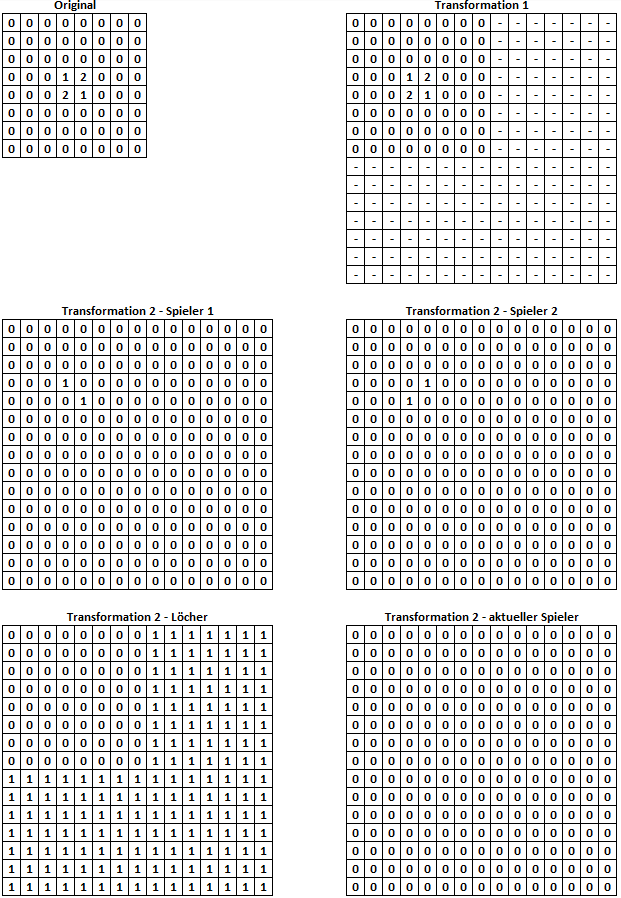
\includegraphics[width=0.8\textwidth]{pics/input_transform.png}	
	\caption{Input-Transformation für das originale Spielfeld, Spieler 1 führt den nächsten Zug aus, eigene Abbildung.}
	\label{fig:input_transformation}
\end{figure}
Einer der wichtigsten Bausteine im machine learning ist der Umgang mit dem Input, da dieser auch maßgeblich für den erzeugten Output ist und vom Modell akzeptiert werden muss. Bei der Evaluierung des NN für einen gegebenen Zustand sind die Spielfeldgröße, die Lage der Spielsteine, eventuelle Löcher und der aktuelle Spieler bekannt. Diese Informationen werden genutzt, um einen einheitlich aussehenden Input für das Modell zu generieren. Dabei wird die Klasse \texttt{PlaygroundTransformer} zur Hilfe genommen. Die entsprechenden Transformationen sind in Abbildung \ref{fig:input_transformation} dargestellt. Hierbei repräsentiert eine \glqq{}0\grqq{} ein freies Spielfeld, ein \glqq{}-\grqq{} signalisiert, dass dieses Feld nicht existiert. Die Ziffern \glqq{}1\grqq{} und \glqq{}2\grqq{} geben an, dass auf der jeweiligen Position ein Spielstein des entsprechenden Spielers liegt.

%TODO
%Bis auf in \glqq Transformation 2 - nächster Spieler\grqq{} repräsentiert eine 0 ein "nicht vorhanden", während ein Strich '-' darstellt, dass dieses Feld nicht existiert. Die Ziffern 1 und 2 geben an, ob der zugehörige Spieler an der gegebenen Position einen Spielstein besitzt. In der \glqq Transformation 2 - nächster Spieler\grqq{} zeigen die 0en an, dass Spieler 1 am Zug ist, bei Spieler 2 wären hier nur 1en dargestellt.

Für die Transformationen definieren wir eine maximale Spielfeldgröße in der Klasse \texttt{AlphaGoZeroConstants} in dem Feld \texttt{DIMENSION\_PLAYGROUND}. Größere Spielfelder können nicht betrachtet werden, kleinere werden am rechten und unteren Rand mit Löchern aufgefüllt, bis die angegebene Spielfeldgröße erreicht wurde.
Auf diesem resultierenden Spielfeld führen wir eine weitere Transformation durch, indem wir das Spielfeld aus mehreren Sichten betrachten, die wiederum die Dimensionen des resultierenden Spielfeldes haben. Die ersten beiden Sichten zeigen auf, an welchen Positionen die beiden Spieler ihre Spielsteine haben. So werden zwei virtuelle Spielfelder erzeugt, die an jeder Position eine 0 haben, außer wenn der jeweilige Spieler einen Spielstein auf der abgefragten Position besitzt, in diesem Fall wird der Wert auf \glqq{}1\grqq{} gesetzt. Die dritte Sicht beschäftigt sich mit den Löchern auf der Karte und setzt eine \glqq{}1\grqq{}  an die Positionen, an denen sich Löcher befinden. Die vierte Sicht schreibt an jede Position entweder eine \glqq{}0\grqq{} , falls Spieler 1 am Zug ist, oder eine \glqq{}1\grqq{}, falls Spieler 2 den nächsten Zug ausführt. Diese vier Sichten werden anschließend in einem \texttt{INDArray} konkateniert und an das Modell übergeben. Diese Transformationen sollen dem NN helfen, die aktuelle Spielsituation korrekt zu bewerten. \bigskip

\subsubsection{Modell}
Das Modell entspricht einem Computation Graph, also einem gerichteten Graphen, bei dem die Knoten entweder Rechenoperationen oder Variablen entsprechen. Das Modell ist sehr tief und wird daher für die Beschreibung in vier Teilblöcke aufgeteilt: den Convolutional-Block, den Residual-Tower, den Policy-Head und den Value-Head. \\
Der Convolutional-Block, der den transformierten Input erstmalig annimmt, besteht aus einem 3-dimensionalem Convolutional-Layer mit einer Kernel-Größe von 3 und einem Stride von 1 analysiert und einen Output mit 256 Dimensionen generiert. Die Werte werden anschließend mit Hilfe der Batchnormalisierung normalisiert, bevor die LeakyRelu-Funktion auf das Ergebnis angewendet wird, um kleine Werte abzuschwächen, sodass größere Werte an Bedeutung gewinnen (siehe linearer Verlauf im positiven). \\
Der Residual-Tower sollte nach \cite{Silver2017} aus 20 bis 40 Blöcken bestehen, je mehr Blöcke verwendet werden, desto länger dauert das Training des Netzes, desto besser soll jedoch auch die zu erwartende Leistung sein. Um langfristig eine möglichst starke KI zu erhalten, haben wir uns auf die 40-Block-Variante geeinigt und diese umgesetzt. Der erste Block entspricht dem Convolutional Block, alle weiteren Blöcke sind ähnlich aufgebaut. Für diese werden jeweils ein Convolutional Block und ein Convolutional Block ohne Aktivierungsfunktion genutzt, für die derselbe Input verwendet wird. Das Ergebnis beider Teilblöcke wird elementweise addiert, sodass die ursprüngliche Eingabe so lange wie möglich erhalten bleibt. Auf den resultierenden Vektor wird danach nochmals die Leaky-Relu-Funktion angewendet. Daraus resultieren (1 + 39*2 = 79) Anwendungen des Convolutional Filters, um die Spielsituation zu analysieren. \\
Das Ergebnis aus dem Residual-Tower wird als Input für die verbleibenden zwei Blöcke genutzt: der Policy-Head und der Value-Head. Der Policy-Head führt einen weiteren Convolutional Filter auf dem Ergebnis aus, dabei werden die Kerne von 256 auf 2 reduziert. Auf dem Resultat  wird eine Batch-Normalisierung und die Leaky-Relu-Aktivierung ausgeführt, bevor dieses in einer Fully-Connected-Layer, bei der jeder Knoten der vorherigen Schicht mit jedem Knoten der aktuellen Schicht verbunden ist, in einen Vektor der Länge 226 transformiert wird, welcher der Anzahl der Spielfelder plus eins (für kein möglicher Zug) entspricht. Auf diesen Output wird beim Training der Cross-Entropy-Fehler berechnet, um die Wahrscheinlichkeit der korrekten Prognose des besten Zuges bestmöglich zu lernen. Alle Werte entsprechen nun den Wahrscheinlichkeiten für die verschiedenen Züge mit den Werten zwischen 0 und 1. Auf dieses Ergebnis wird in der Klasse \texttt{PolicyValuePredictor} zudem die Dirichlet-Funktion angewendet, diese verstärkt große Werte und schmälert die Werte für schlechtere Züge, mit der Wahl des Parameters $\theta$ kann man jedoch noch einen Temperaturparameter angeben. Liegt dieser Parameter bei $>= 1$ wird das berechnete Ergebnis so ausgegeben wie es ist. Bei Werten zwischen 0 und 1 werden manche Züge deutlich verstärkt, wobei dies auch Züge sein können, die zuvor einen schlechten Prognosewert hatten. Je weiter der Wert von 1 entfernt liegt, desto wahrscheinlicher wird es, nicht den Zug mit dem besten Prognosewert zu wählen. Als Ergebnis erhält man wieder einen Vektor, dessen Werte sich zwischen 0 und 1 befinden und sich auf 1 addieren. Dieses Feature soll die Exploration während der Lernphase erhöhen indem Zufallszüge zugelassen werden, ansonsten wird immer der gleiche Spielablauf ersichtlich, womit der Lernversuch keine Erfolge mehr schafft. Mithilfe der Wahl eines festen Parameters $\theta$ haben wir mehrmals dasselbe Spielergebnis erhalten, eine Verbesserung gab sich erst, als zu Spielbeginn zufällig ein Wert  $\theta$ aus den verschiedenen willkürlichen Werten $\{0,1; 0,2; 0,4; 0,8\}$ ausgewählt wird, mit denen tendenziell eine höhere Exploration erreicht wird. Außerhalb von Lernzyklen wird $\theta$ auf 1 gesetzt, um keine zufällige Exploration zuzulassen und somit stabiler zu sein, somit kann diese KI als Referenz gegenüber der lernenden KI genutzt werden. \\
Als letzten größeren Block betrachten wir den Value-Head. Der Value-Head besteht, wie zunächst auch der Policy-Head aus einem Convolutional-Filter, der die 256 Kerne auf einen Kern reduziert (in diesem sind nun 15x15 Werte vorhanden), einer Batchnormalisation, der Aktivierung mittels LeakyRelu sowie zwei Fully-Connected-Schichten. Bei der letzten Schicht wird das Endergebnis auf einen Wert reduziert, welches mittels der Tangenshyperbolicus-Funktion ein letztes Mal angepasst wird. Um die Abweichung der Prognose des Value-Heads im Training vom Soll zu ermitteln, um damit die realen Parameter anpassen zu können, wird der MSE verwendet. 

\subsubsection{Grundlegende Konfiguration}
Die Klasse \texttt{NeuronalNet} beinhaltet neben dem Modell des NN, die grundlegende Konfiguration. Hierzu gehören das Momentum mit einem Wert von 0,9, der Optimierungsalgorithmus \glqq{}Stochastic Gradient Descent\grqq{} bei dem pro Trainingsiteration eine Batchgröße von 1 verwendet wird und die L1-Regularisierung, die auf den Wert 0,9 gesetzt wird. Des Weiteren werden an dieser Stelle weitere Optionen konfiguriert, wie die Nutzung der Backpropagation, die Initialisierung der Gewichte im NN, die DeepLearning4J im Gegensatz zur Angabe im Paper nicht zufällig initialisieren kann, daher verwenden wir hier die He-Initialisierung
\begin{equation}
Var(w_i) = \frac{2}{fan\_in}
\end{equation}
als eine Erweiterung der Xavier-Initialisierung, die sich gut mit tiefen neuronalen Netzen und der Relu-Aktivierungsfunktionen verträgt \cite{Ghatak.2019}. Hierbei ist der Wert des Gewichts abhängig von der Anzahl der eingehenden und ausgehenden Neuronen, somit sind die Werte im weitesten Sinne auch wieder zufällig gewählt und konvergieren beim Training sowieso gegen das Optimum. Die Lernrate orientiert sich am genannten Paper, hierfür kann in DeepLearning4J keine automatische Anpassung integriert werden. Da wir Probleme mit der Berechnung auf der GPU haben und somit nur auf der CPU rechnen, betrachten wir die Lernraten für wenige Spiele. Hierfür werden die Werte zwischen 0,1 und 0,001 empfohlen, nach Tests mit jeweils 50 Spielen hat die Lernrate von 0,01 als einzige von 8 getesteten Werten Lernerfolge vorgewiesen, weshalb wir diesen Wert fest integriert haben. Die L2-Regularisierung, die den Effekt des Overfittings verringern soll, ist abhängig davon, ob der Policy Head oder der Value Head betrachtet wird. Zu Beginn wurde die Regularisierung für beide Komponenten, wie im Paper vorgeschlagen auf einen Wert von $10^{-4}$ gesetzt. Infolgedessen nahmen die Werte des Value Heads nach jedem Training einen neuen Wert an, von dem, bis zum nächsten Training, kaum mehr abgewichen wurde, wodurch alle Zustände fast identisch bewertet wurden. Um dieses Problem zu beheben, wurde der Wert der L2-Regularisierung des Value Heads stufenweise erhöht. Ab einem Wert von $10^{-3}$ ist eine leichte Dämpfung des beschriebenen Effekts erkennbar, bei $10^{-2}$ wirkt die Lerngeschwindigkeit annehmbar und bei $10^{-1}$ verändert sich die Prognose mit jedem Training nur minimal und ist somit auch nicht zu gebrauchen. Aus diesem Grund haben wir den Wert der L2-Regularisierung des Policy Heads auf $10^{-2}$ eingestellt.\\
Die empfohlene Batchgröße von 8 konnte nicht verwendet werden, da DeepLearning4J Batches derzeit nicht in Kombination mit mehreren Outputs zulässt. Durch die Wahl des Stochastic Gradient Descent Optimierungs-Algorithmus wird generell jeder Datensatz einzeln für die Optimierung herangezogen. Die einzige erkennbare Auswirkung wäre im Bereich der Batchnormalisierung zu finden gewesen, diese sollte durch die große Anzahl an Spielen keinen nennenswerten Einfluss auf das Endergebnis haben, jedoch ist es möglich, dass eine längere Lerndauer benötigt wird. 

\subsubsection{Schwierigkeiten}
Wie bei allen NN wird auch hier zuerst das Modell aufgebaut und kompiliert, bevor der Input an das Modell übergeben wird. Durch die Tiefe des Netzes sind Fehler oft nur nach intensiver Suche zu finden. Zudem gibt DeepLearning4J aufgrund der Struktur nur sehr notdürftige Fehlermeldungen aus. Diese lassen zwar einen Rückschluss auf das Problem (wie beispielsweise Fehler in der Definition der Dimensionen) zu, geben jedoch die genaue Quelle nicht an. Dies machte den initialen Aufbau des Modells zu einem langwierigen Prozess, da mit einem sehr einfachen Modell gestartet werden musste, welches nur langsam erweitert werden konnte. Hierfür muss jedoch auch jeweils die zugehörige Output-Schicht adaptiert werden, wobei ebenfalls Fehler auftreten können.\\
Ein weiteres Problem lag im Optimieren der Hyperparameter. Da DeepLearning4J nicht alle benötigten Funktionen, wie für das zufällige Initialisieren der Gewichte oder das Fehlen der Batchnormalisierung für mehrere Outputs, zur Verfügung stellt, musste an dieser Stelle eine Adaption gefunden werden, was sich teils sehr schwierig gestaltet hat. 


\newpage

% ----------------------------------------------------------------------------------
% Kapitel: Training
% ----------------------------------------------------------------------------------

\section{Training des neuronalen Netzes}
Um die KI lernen zu lassen, ist das Training der zentrale Punkt, um eine Optimierung des Spielverhaltens zu erreichen, sodass die KI immer stärkere Gegner besiegen kann.  Hierfür werden zwei Komponenten benötigt, einerseits wie das Training des Modells innerhalb des Programms aussehen soll, und andererseits, da das Programm für das Training gegen seine aktuell beste Version spielen soll, ein externes Skript, dass eine Serie von Spielen und verwaltet. Das Shell-Skript mit dem Namen *\_multigame.sh \footnote{Fundort: \url{https://gitlab.oth-regensburg.de/kec39902/hsp-ws19-g03-reversiml/-/tree/master/ReversiXT_Tools/Scripts/multigame}}, wobei der Asterisk für das verwendete Betriebssystem steht, gliedert sich in folgende Teile: Löschen von veralteten Log-Dateien, Schleife welche definiert, wie viele Spielserien mit je zwei Spielen ausgeführt werden und in der die benötigten Komponenten zwei Mal aufgerufen werden, bei einem Spiel startet die lernende KI als Spieler 1 und einmal als Spieler 2, um nicht spezifisch Spieler 1 oder Spieler 2 zu lernen. Nach jedem einzelnen Spiel erfolgt eine Wartezeit, bis die lernende KI den Trainingsvorgang abgeschlossen hat. Wichtig zu wissen ist, dass wenn keine Grafikkarte genutzt wird oder diese Nutzung nicht richtig funktioniert, in der pom.xml des AlphaZero-Clients die zwei Dependencies, die sich auf Cuda beziehen (erkennbar an der Zeile mit der genannten Cuda-Version) auskommentiert werden. Ebenfalls muss in der \texttt{Main}-Klasse in der \texttt{main}-Funktion die Erlaubnis für die Verwendung von mehreren Grafikkarten \texttt{CudaEnvironment.getInstance().getConfiguration().allowMultiGPU(true)} auskommentiert werden, ebenso der Import der \texttt{CudaEnvironment}. \\
Der Aufbau des Trainings innerhalb der KI erfolgte in mehreren Etappen, die im Folgenden beschrieben werden. Der erste Versuch war, dem neuronalen Netz bei guten Zügen einen Bonus zu übergeben, damit sich diese verbessern kann. Für DeepLearning4J konnte mit dem gewählten Modell jedoch kein geeigneter Ansatz implementiert werden, da das Netz für mehrere Outputs keine Rewards annehmen kann. Auf der Suche nach einer Lösung haben wir in \cite{Silver2017} die Möglichkeit gefunden, vom Reinforcement Learning abzuweichen und setzten stattdessen auf den Supervised-Learning-Ansatz, indem wir in jedem Spiel eine Historie aufbauen, und das Modell am Ende des Spiels nachzutrainieren. Auch hierfür gab es zwei Varianten, in beiden speichern wir für jeden real gespielten Spielzug den aktuellen Spieler, den Spielzustand, den angepassten Policy Head, der vom MCTS generiert wird und den angepassten Value Head, mit den Werten -1 bei Verlust, 0 bei Patt und 1 bei Gewinn des Spiels. Somit erhalten wir nach jedem Spiel auf einem 8x8 Brett bis zu 60 Datensätze für das Training. Im ersten Versuch spielten wir immer fünf Spiele, nach welchen entschieden wurde, ob das aktuelle Modell mit 55\% Siegquote besser ist als das bisherige beste Modell oder nicht. Parallel dazu wurde ein weiteres Modell nach jedem Spiel vortrainiert, welches das aktuelle Modell ersetzen sollte. Dieses wurde benötigt, damit sich das aktuell spielende Modell nicht verändert und somit eine Aussage, ob das Modell besser beziehungsweise schlechter als das bisherige beste Modell ist, gewährleistet werden kann. Als Ergebnis erhielten wir jedoch innerhalb der fünf Spiele nur identische Spielverläufe, eventuell auch dem geschuldet, dass zu diesem Zeitpunkt die Dirichlet-Funktion nicht implementiert war. Aufgrund dessen haben wir die 55\% Quote ignoriert und das Modell nach jedem Spiel direkt trainiert und mit dem besten Modell verglichen. Das Risiko ist hierbei jedoch, dass das Lernen um einen Punkt oszilliert, anstatt sich deutlich zu verbessern. Diesem Aspekt hoffen wir mit genug Trainingsspielen und einem hohen Zufallsfaktor $\theta$ in der Dirichlet-Funktion entgegenzuwirken. Die Erfahrung ist nach ca. 5000 gespielten Spielen, dass hier eine deutliche Verbesserung stattfindet, da unsere AlphaZero, unter der Bedingung, dass unsere KI als zweites startet, die triviale KI bis zu einer Suchtiefe des Wertes sechs besiegen kann. Zudem gewinnen wir auf einer Suchtiefe von drei, wenn wir als erstes starten. Die niedrige Anzahl von 5000 Trainingsspielen erklärt sich über die hohe benötigte Laufzeit, denn ein Spiel dauert bei der Berechnung auf der CPU ungefähr drei Minuten für das Spiel und weitere fünf Minuten für das Nachtrainieren der KI. Zu Beginn des Trainings war beides noch nicht möglich. Bei gespielten 5000 Spielen ist dieses Ergebnis bereits annehmbar, wenn man bedenkt, dass die originale AlphaZero mehrere Millionen Spiele spielte. Zudem traten hin und wieder Probleme beim Training auf, wie ein Stopp aufgrund fehlender Speicherressourcen, oder dass die Programmkomponenten nach einer zufälligen Anzahl Iterationen nicht mehr im Prozessverzeichnis als laufende Prozesse registriert waren (Ermittlung mittels: ps -ef\:  \textbar\: grep \glqq Name-der-Programmkomponente\grqq{}). Diese Fehler konnten, da diese zu willkürlichen Zeitpunkten auftraten nicht nachgestellt werden. Die Vermutung liegt jedoch bei der Speicherfreigabe des \texttt{ScheduledThreadPoolExecutors}, der die Spielzüge zeitlich terminiert, sowie ein daraufhin möglicherweise administratives Entfernen der zugehörigen Prozesse. \\
Das Training erfolgte mit mehreren Problemen, da auf der gestellten Workstation, die Nutzung der Grafikkarten nicht möglich war. Auf einem eigenen Rechner funktioniert dies jedoch, die Unterschiede in der Nutzung sind hierbei das installierte Betriebssystem: Ubuntu 18.04 vs Ubuntu 18.04 LTS und die Version des Grafikkartentreibers: Nvidia-435 vs Nvidia-440. Jedoch war auf dem eigenen Rechner nur eine Grafikkarte vorhanden, weshalb ein Training des Modells gegen das beste Modell nicht möglich war, da hier bereits ein Modell den Speicher auf der Grafikkarte fast komplett belegt. Das Berechnen und Lernen auf der CPU kostet jedoch einiges mehr an Zeit, weshalb verhältnismäßig nur wenige Spiele gespielt werden konnten. Möglicherweise hätte hier eine noch bessere Abstimmung mit dem Administrator Prof. Kern geholfen, um entweder den korrekten Grafikkartentreiber installieren zu können oder die Komponenten für eine ältere Version downzugraden.

\newpage

% ----------------------------------------------------------------------------------
% Kapitel: Ergebnis/Endzustand/Funktionsumfang
% ----------------------------------------------------------------------------------
\section{Endergebnis}
%TODO Zusammenfassen, was kann das Spiel alles
Als abschließendes Ergebnis lässt sich festhalten, dass das Programm gelernt hat Reversi auf einem quadratischen Feld der Größe 15x15 zu lernen. Gegen die von Prof. Kern zur Verfügung gestellte triviale KI wird dabei zu X\% gewonnen. 

Um das Spiel etwas interessanter und f\"{u}r unsere KI etwas herausfordernder zu gestalten, lassen wir derzeit Spielfeldgr\"{o}\ss en bis zu 15x15 Feldern zu, die Startposition der Anfangssteine darf hierbei beliebig sein und muss nicht mittig angelegt werden. Gr\"{o}\ss ere Spielgr\"{o}\ss en k\"{o}nnen in der Klasse \texttt{AlphaGoZeroConstants} in der Konstante \texttt{DIMENSION\_PLAYGROUND} gesetzt werden, der hierf\"{u}r ben\"{o}tigte Wert ist das Maximum aus der Spielfeldh\"{o}he und der -breite. Bei einer \"{A}nderung muss jedoch das Modell von Grund auf neu trainiert werden.\\
Zudem lassen wir sogenannte L\"{o}cher im Spielfeld zu, also Felder auf die keiner der Spieler ziehen kann. Das Setzen auf anliegende Felder ist somit sicherer als mittig im Spielfeld, da die Spielsteine nicht vom Feld des Loches aus umgekehrt werden k\"{o}nnen.


\newpage

% ----------------------------------------------------------------------------------
% Kapitel: Allgemeine Informationen/Organisation
% ----------------------------------------------------------------------------------
\section{Organisation}

\subsection{Team und Aufgabenverteilung}
% Beschreiben Sie in diesem Abschnitt Ihr Team. Welche Person hat welche Aufgaben wahrgenommen, wie wurden
% Aufgaben aufgeteilt und wie wurde kommuniziert, etc.
Als Dreier-Team bestand unsere Gruppe aus Simon Hofmeister, Monika Silber und Simon Wasserburger. Anfangs war zusätzlich Nadiia Matsko Teil unseres Teams, jedoch beendete sie das Projekt vorzeitig. Sie war daher beim Schreiben der Unterpunkte  \ref{secAlphaGo} und \ref{secAlphaZero} sowie bei der initialen Implementierung des NN mit involviert. Anzumerken ist, dass Simon Hofmeister und Simon Wasserburger bereits im Bachelorkurs Erfahrung mit dem Implementieren einer künstlichen Intelligenz für Reversi sammeln konnten. Aus diesen Gründen griffen wir für den Aufbau dieses Projektes auf das Grundgerüst des bereits im Bachelorkurs erstellen Programms von Simon Hofmeister zurück, der dieses entsprechend an die Anforderungen des vorliegenden Projektes anpasste.

Hinsichtlich der Verteilung der Aufgaben und des zugehörigen Aufwands ergab sich für die einzelnen Teammitglieder folgendes:

\begin{tabular}{*{3}{p{4cm}p{3cm}p{8cm}}}
\multicolumn{3}{l}{\textbf{Simon Hofmeister (150 h):}} \\
Bereiche & Zeitaufwand & Komponenten \\
\cline{1-3}
Recherche & 30 Std &  \\
Implementierung & 80 Std & Grundgerüst, NN, Installation, Script Training  \\
Dokumentation & 10 Std & Implementierung NN, Training des NN, Testumgebungen und Installation \\
Organisation & 30 Std &  Besprechungen\\
\end{tabular}


\begin{tabular}{*{3}{p{4cm}p{3cm}p{8cm}}}
\multicolumn{3}{l}{\textbf{Monika Silber (150 h):}} \\
Bereiche & Zeitaufwand & Komponenten \\
\cline{1-3}
Recherche & 40 Std &  \\
Implementierung & 40 Std & MCTS, Vorbereitung Training  \\
Dokumentation & 40 Std &  Einleitung, Theoretische Grundlagen, Implementierung MCTS, Organisation \\
Organisation & 30 Std &  Besprechungen\\
\end{tabular}


\begin{tabular}{*{3}{p{4cm}p{3cm}p{8cm}}}
\multicolumn{3}{l}{\textbf{Simon Wasserburger (130 h):}} \\
Bereiche & Zeitaufwand & Komponenten \\
\cline{1-3}
Recherche & 20 Std &  \\
Implementierung & 70 Std & MCTS, Code-Refactoring Grundgerüst  \\
Dokumentation & 10 Std &  Grafiken MCTS, Aufbau des Programms \\
Organisation & 30 Std &  Besprechungen\\
\end{tabular}

\subsection{Kommunikation}
Die virtuelle Kommunikation fand hauptsächlich in unserer WhatsApp-Gruppe statt, wo wir einander auf Problemstellen aufmerksam machten, Lösungsansätze diskutierten, einander über Fortschritte informierten und Treffen ausmachten. Ebenfalls konnte durch Commits im Repository die Arbeit der Teamkollegen und entsprechend der Projektfortschritt verfolgt werden. Daneben verfügten wir über ein Trello-Board, in dem wir Aufgaben planten, dokumentierten und zuwiesen. In gemeinsamen Treffen besprachen und ergänzten wir dabei die offenen Punkte und kontrollierten den Projektablauf. 

In den persönlichen Treffen, in denen meist alle Teammitglieder anwesend waren, konnten wir alle offenen Punkte konkretisieren und ausführlich diskutieren. Wir erarbeiteten gemeinsame Lösungsstrategien und halfen einander bei Verständnisproblemen. Abschließend trafen wir Absprachen zum weiteren Vorgehen sowie zur Aufgabenverteilung. In Ausnahmefällen erfolgte dies online per Sprachkonferenzen.

\subsection{Versionskontrolle}
Als Versionskontrollsystem stand ein Gitlab-Repository der OTHR zur Verfügung. Zum Abrufen und Bearbeiten dessen wurde GitHub Desktop als GUI verwendet.
%TODO welche GUI/CLI?

Hinsichtlich Implementierung der Komponenten wurden eigene Branches angelegt, die vom master-Branch geklont und nach Fertigstellung entsprechend dort wieder gemergt wurden. Dabei ergaben sich eigene Branches für den MCTS, das NN sowie für den Prozess des Refactoring des ursprünglichen Codes. Die finale und alle Bestandteile umfassende Version befindet sich folglich im master-Branch.

\subsection{OS, IDE und Programmiersprache}
%TODO OS
Als Entwicklungsumgebung wurde IntelliJ IDEA\footnote{https://www.jetbrains.com/de-de/idea/} von JetBrains genutzt. Da wir innerhalb der Gruppe bisher am meisten Erfahrung in Java hatten, wurde dies als Programmiersprache zur Implementierung des Projektes verwendet. Zur Erstellung des Programms kam maven\footnote{https://maven.apache.org/} als Build-Management-Tool zum Einsatz.

Des Weiteren wurde zur Implementierung des NN die Library Eclipse deeplearning4j (DL4J) \cite{DL4J} zur Hilfe genommen. Hinsichtlich dieser Auswahl verschafften wir uns zunächst einen Überblick über vorhandene, gute Bibliotheken und recherchierten deren Vorteile und Anwendungsfälle, wobei die Entscheidung letztendlich auf die bereits genannte fiel.

Da wir uns innerhalb der Gruppe auf die Programmiersprache Java geeignet hatten, suchten wir dementsprechend eine deep-learning-Library für Java. Zwar stellt beispielsweise das bekannte Python-Framework TensorFlow\footnote{https://www.tensorflow.org/} eine Java API bereit, diese besitzt jedoch experimentellen Charakter\footnote{$https://www.tensorflow.org/api_docs/java/reference/org/tensorflow/package-summary$} und ist daher für unsere Zwecke ungeeignet. 

Ebenfalls die beliebte Python-Bibliothek Keras\footnote{https://keras.io/} bietet Möglichkeiten zur Anbindung an Java. Zwar können in Keras trainierte Modelle mithilfe von DL4J nach Java importiert werden, jedoch müssen diese zuvor in Python konfiguriert und trainiert werden\footnote{https://deeplearning4j.org/docs/latest/keras-import-overview}.

Jython ist eine Bibliothek, die es erlaubt Python-Code in Java-Umgebungen zu schreiben und somit einfach zu integrieren, jedoch ist nicht klar, ob die benötigten Bibliotheken ebenfalls auf der Java-Plattform ausgeführt werden können, zudem erscheint uns diese Variante sehr langsam, da die DeepLearning sehr rechenintensiv ist und die Nutzung der Java-Plattform dies ausbremsen könnte.

Da DL4 hinsichtlich unserer individuellen Projektansprüche am besten schien, fiel die Entscheidung letztlich auf diese Wahl. Entsprechend folgt nun die Darlegung der Eigenschaften von DL4J, wobei der Fokus auf der Ausarbeitung der für das vorliegende Projekte relevanten Aspekten liegt. Sämtliche Informationen sind, sofern nicht anders angegeben, der zugehörigen Website (https://deeplearning4j.org/) entnommen.

Die Library hat ihren Ursprung bei Entwicklern der Firma Konduit\footnote{https://konduit.ai/} in San Francisco und wurde unter der Apache Software Foundation License 2.0\footnote{https://www.apache.org/licenses/LICENSE-2.0} veröffentlicht.

DL4J ist vollständig open source und in Java geschrieben, wobei für die zugrundeliegenden Berechnungen C, C++ und Cuda genutzt wurden. Des Weiteren unterstützt sie ND4J (N-Dimensional Arrays for Java) - eine Bibliothek für das wissenschaftliche Rechnen, die eine hohe Performanz gewährleistet\footnote{https://nd4j.org/}. Diese werden im vorliegenden Projekt anhand von \texttt{INDArrays} referenziert.
%TODO INDArrays

Außerdem werden zahlreiche, hilfreiche Features unterstützt, unter anderem Batch Normalisation, Residual Learning, CNNs. In Form eines \texttt{ComputationGraph} kann daher ein verhältnismäßig einfach ein komplexes neuronales Netz aufgebaut werden.

Weitere ausschlaggebende Vorteile liegen in der ausführlichen Dokumentation\footnote{https://deeplearning4j.org/api/latest/} sowie den zahlreichen Hilfsmitteln, wie Tutorials\footnote{erreichbar über https://deeplearning4j.org/tutorials/setup}, Code-Beispiele\footnote{https://github.com/eclipse/deeplearning4j-examples} und Leitfäden zu sämtlichen Aspekten\footnote{erreichbar über https://deeplearning4j.org/docs/latest/}, die zudem alle schnell und unkompliziert über die eigene Website zu finden sind.

Zuletzt können wir nach Projektabschluss festhalten, dass wir DL4J als sehr benutzerfreundlich und unkompliziert empfanden. Ebenfalls der große Funktionsumfang erleichtert die Arbeit zum Aufbau und Training des Modells. Daher sehen wir DL4J insgesamt als hilfreiches und anwenderfreundliches Tool.

%TODO Alternativen, abschließenden Bewertung (Kritikpunkte?)

\subsection{Testumgebungen und Installation}
Um die Leistungen des Trainings der implementierten AlphaZero einschätzen oder nachbauen und nutzen zu können, ist es wichtig, sich mit den Rahmenbedingungen des Projektes zu beschäftigen. Hierzu werden im Folgenden die technischen Daten des Projektes wiedergegeben und die Installation der benötigten Komponenten erläutert.

\subsubsection{Testumgebungen}
Die hauptsächlich genutzte Umgebung, ist die von der OTH Regensburg gestellte Workstation vom Typ Alienware Aurora R7. Dieser Besitzt einen Intel i7-8700K Prozessor mit 3,7GHz Taktung, 6 Kernen mit 12 möglichen Threads und AVX2-Support. Der RAM entspricht 64GB-DDR4-Speicher, zudem sind 2 Nvidia GTX 1080 TI integriert. Installiert sind neben dem Betriebssystem Ubuntu 18.04 (64-Bit) das OpenJDK in der Version 11.0.6, Maven als Build-Tool, Git, Cuda in der Version 10.2, Cudnn in der Version 7.6.5 und der Grafikkartentreiber in der Version Nvidia-435.

Zudem erfolgten Tests auf einem weiteren Rechner mit einem i7-6700K Prozessor mit 4GHz Taktung, 4 realen Kernen und AVX2-Support, 32GB-DDR4-RAM sowie einer Nvidia GTX 1060 (6GB GDDR5-RAM). Installiert sind neben dem OS Ubuntu 18.04 LTS hierauf dieselben Tools, wie auf der Workstation, nur dass sich hier der Grafikkartentreiber unterscheidet, dieser ist hier in der Version Nvidia-440 installiert. 

%TODO: Installation
\subsubsection{Installation}
Für die Kompilierung des Quellcodes werden eine Java-Runtime in der Version $>= 1.8$ und Maven benötigt. Für die Ausführung auf der Grafikkarte wird das Cuda-Toolkit mit dem passenden Grafikkartentreiber benötigt. Optional kann CuDNN für eine weitere Beschleunigung installiert werden.
\begin{table}
\begin{tabularx}{\textwidth}{ | X | X | X | }
	\hline
	\textbf{Cuda-Version} & \textbf{Cudnn-Version} & \textbf{Grafikkarten-Treiber} \\
	\hline \hline
	10.2 & 7.6 & 440 \\
	10.1 & 7.6 & 418.39 \\
	10.0 & 7.4 & 410.48 \\
	9.2 & 7.2 & 396.26 \\ \hline
\end{tabularx}	
\caption{Aktuell kompatible Versionen von DL4J mit Cuda, Cudnn \cite{DL4JCUDNN} und dem Grafikkartentreiber \cite{NVIDIACUDNN} für die Nvidia GTX 1080TI Grafikkarten.}
\label{tab:cuda-cudnn}
\end{table}

Im Folgenden wird die Installation der benötigten Komponenten im Detail erklärt. Zu Beginn wird für Java das OpenJDK, danach Maven sowie bei Grafikkartenverwendung Cuda und optional Cudnn installiert. Anschließend daran befindet sich eine kurze Einführung in das Texteditor-Programm vi, welches auf Linux-Umgebungen genutzt werden kann, um die benötigten Dateiänderungen durchzuführen.\\

Bevor die Installation an sich beginnt, werden die Pakete des Paketmanagers auf den neuesten Stand gebracht.
\begin{flalign*}
& \hspace{-5.4 cm} \text{sudo apt-get update} \\
& \hspace{-5.4 cm} \text{sudo apt-get upgrade} \\
& \hspace{-5.4 cm} \text{sudo apt-get autoremove} \\
\end{flalign*}
Möglicherweise wird im Folgenden ein erneuter Login benötigt, falls eine Datei im Verzeichnis /lock/var/lib/dpkg/ weiterhin gesperrt ist. \\
Nun kann die Installation des OpenJDKs erfolgen. 

\begin{flalign*}
& \text{sudo apt-get install default-jdk} \\
& \text{sudo vi /etc/profile} \\
& \hspace{1 cm} \text{Um folgenden Inhalt erweitern:} \\
& \hspace{1 cm} \text{export JAVA\_HOME=/usr/lib/jvm/$<$Java-Ordner$>$}\\
& \hspace{1 cm} \text{export PATH=\$JAVA\_HOME/bin:\$PATH} \\
& \text{// Logout und erneuten Login durchführen.} \\
& \text{// Verifizierung der Installation:} \\
\end{flalign*}
\begin{flalign*}
& \text{echo \$JAVA\_HOME // Ausgabe: der gewollte Java-Pfad} \\
& \text{Java --version // Ausgabe: Java-Version größer 1.8}
\end{flalign*}

Der nächste Schritt gilt der Installation des Build-Management-Tools Maven, der für die Kompilierung des Quellcodes benötigt wird, um die ausführbare jar-Datei zu erhalten.
\begin{flalign*}
& \hspace{-2.4 cm}\text{sudo apt-get install maven} \\
& \hspace{-2.4 cm}\text{// Verifizierung der Installation:} \\
& \hspace{-2.4 cm}\text{mvn --version // Ausgabe: Maven-Version} \\
\end{flalign*}

Die weiteren Installationen werden nur benötigt, wenn die Berechnungen auf einer oder mehreren Nvidia-Grafikkarten ausgeführt werden sollen. Benötigt wird dafür die Cuda um auf die Cuda-Kerne zugreifen zu können. Hierfür werden zuerst alte Cuda-Versionen entfernt, falls Cuda für weitere Programme benötigt wird, gilt hier der Hinweis, dass Cuda bis einschließlich der Version 10.2 rückwärtskompatibel ist.

\begin{flalign*}
& \hspace{-0.2 cm}\text{sudo apt-get purge nvidia*} \\
& \hspace{-0.2 cm}\text{sudo apt remove nvidia-*} \\
& \hspace{-0.2 cm}\text{sudo rm /etc/apt/sources.list.d/cuda*} \\
& \hspace{-0.2 cm}\text{sudo apt-get autoremove \&\& sudo apt-get autoclean} \\
& \hspace{-0.2 cm}\text{sudo rm -rf /usr/local/cuda*} \\
\end{flalign*}

Als nächstes wird geprüft, ob die Grafikkarte für eine Cuda-Installation geeignet ist, und ob der gcc-Compiler mindestens in der Version 7 (wie von Cuda 10.2 gefordert) vorhanden ist. 

\begin{flalign*}
& \hspace{2.2 cm}\text{lspci | grep -i nvidia // Ausgabe: cuda-kompatible Grafikkarten} \\
& \hspace{2.2 cm}\text{gcc --version // Ausgabe: gcc-Version, sollte größer als 7 sein} \\
\end{flalign*}
\begin{flalign*}
& \hspace{-3.5 cm}\text{// Bei kleinerer GCC-Version: } \\
& \hspace{-3.5 cm}\text{sudo apt-get install gcc} \\
& \hspace{-3.5 cm}\text{gcc --version // erneute Prüfung} \\
\end{flalign*}

Mögliche Änderungen müssen im Paketmanager aktualisiert werden, zudem fehlen noch mehrere Vorbedingungen für die Cuda-Installation, die im nächsten Schritt installiert werden.

\begin{flalign*}
& \hspace{2.3 cm}\text{sudo apt-get update} \\
& \hspace{2.3 cm}\text{sudo apt-get upgrade} \\
& \hspace{2.3 cm}\text{// Logout und erneuten Login durchführen.} \\
& \hspace{2.3 cm}\text{sudo apt-get install gcc} \\
& \hspace{2.3 cm}\text{sudo apt-get install g++ freeglut3-dev build-essential libx11-dev} \\
& \hspace{4.7 cm}\text{libxmu-dev libxi-dev libglu1-mesa libglu1-mesa-dev} \\
\end{flalign*}

Im nächsten Bereich wird der Grafikkartentreiber aktualisiert und Cuda 10.2, inklusive dem Cuda-Toolkit, installiert.

\begin{flalign*}
& \hspace{3.4 cm}\text{sudo add-apt-repository ppa:graphics-drivers/ppa} \\
& \hspace{3.4 cm}\text{sudo apt-key adv --fetch-keys} \\ 
& \hspace{4.1 cm}\text{http://developer.download.nvidia.com/compute/cuda/repos/} \\
& \hspace{4.1 cm}\text{ubuntu1804/x86\_64/7fa2af80.pub} \\
& \hspace{3.4 cm}\text{echo \grqq{}deb https://developer.download.nvidia.com/compute/cuda/} \\
& \hspace{4.1 cm}\text{repos/ubuntu1804/x86\_64 /\grqq{} | sudo tee /etc/apt/sources.list.d/} \\
& \hspace{4.1 cm}\text{cuda.list} \\
& \hspace{3.4 cm}\text{wget https://developer.download.nvidia.com/compute/cuda/repos/} \\
& \hspace{4.1 cm}\text{ubuntu1804/x86\_64/cuda-ubuntu1804.pin} \\
\end{flalign*}
\begin{flalign*}
& \hspace{3.8 cm}\text{sudo mv cuda-ubuntu1804.pin /etc/apt/preferences.d/cuda-repository} \\
& \hspace{4.5 cm}\text{-pin-600} \\
& \hspace{3.8 cm}\text{wget http://developer.download.nvidia.com/compute/cuda/10.2/Prod} \\
& \hspace{4.5 cm}\text{/local\_installers/cuda-repo-ubuntu1804-10-2-local-10.2.89-440.33.01} \\
& \hspace{4.5 cm}\text{\_1.0-1\_amd64.deb} \\
& \hspace{3.8 cm}\text{sudo dpkg -i cuda-repo-ubuntu1804-10-2-local-10.2.89-440.33.01\_1.0-1} \\
& \hspace{4.5 cm}\text{\_amd64.deb} \\
& \hspace{3.8 cm}\text{sudo apt-key add /var/cuda-repo-10-2-local-10.2.89-440.33.01/7fa2af80} \\
& \hspace{4.5 cm}\text{.pub} \\
& \hspace{3.8 cm}\text{sudo apt-get update} \\
& \hspace{3.8 cm}\text{sudo apt-get install nvidia-440 // alternativ kleinere Treiberversion,} \\
& \hspace{4.5 cm}\text{Anpassung an die DL4J kompatiblen Cuda-Versionen siehe Tab. \ref{tab:cuda-cudnn},} \\
& \hspace{4.5 cm}\text{Anpassung in der pom.xml des Reversi-Clients} \\
& \hspace{3.8 cm}\text{sudo apt-get update} \\
& \hspace{3.8 cm}\text{// Logout und erneuten Login durchführen.} \\
& \hspace{3.8 cm}\text{sudo apt-get -o Dpkg::Options::=\grqq{}--force-overwrite\grqq{} install cuda cuda-} \\
& \hspace{4.5 cm}\text{drivers} \\
& \hspace{3.5 cm}\text{sudo vi /etc/profile} \\
& \hspace{4.8 cm}\text{Um folgenden Inhalt erweitern:} \\
& \hspace{4.8 cm}\text{export PATH=/usr/local/cuda-$<$cuda-version$>$/bin:\$PATH} \\
& \hspace{4.8 cm}\text{export LD\_LIBRARY\_PATH=/usr/local/cuda-$<$cuda-version$>$/} \\
& \hspace{4.8 cm}\text{lib64:\$LD\_LIBRARY\_PATH} \\
& \hspace{4.8 cm}\text{export CUDA\_PATH=/usr/local/cuda-$<$cuda-version$>$} \\
& \hspace{3.8 cm}\text{// Logout und erneuten Login durchführen.} \\
& \hspace{3.8 cm}\text{sudo ldconfig} \\
& \hspace{3.8 cm}\text{sudo apt-get -o Dpkg::Options::="--force-overwrite" install nvidia-cuda-} \\
& \hspace{4.5 cm}\text{toolkit} \\
\end{flalign*}

Falls es gewünscht ist, die Rechenzeit bestmöglich zu optimieren, kann zusätzlich das CuDNN Paket installiert werden.
In dieser Anleitung wird CuDNN 7.6.5 als kompatible Version zu Cuda 10.2 verwendet, siehe Tab. \ref{tab:cuda-cudnn}. Für den Download von CuDNN muss man sich kostenlos für das Cuda-Developer-Programm anmelden.

\begin{flalign*}
& \hspace{4 cm}\text{Website: \url{https://developer.nvidia.com/cudnn}} \\
& \hspace{4 cm}\text{Klick auf Download CuDNN} \\
& \hspace{4 cm}\text{Registrieren / Anmelden} \\
& \hspace{4 cm}\text{Download von Cudnn 7.6.5 als tar-Datei für Linux} \\
& \hspace{4 cm}\text{Zip Datei speichern} \\
& \hspace{4 cm}\text{cd /home/$<$user$>$/Downloads} \\
& \hspace{4 cm}\text{tar -xzvf $<$cudnn-tar-Datei$>$  // wie: cudnn-10.2-linux-x64-v7.6.5.32.tar} \\
& \hspace{4 cm}\text{sudo cp -P cuda/include/cudnn.h /usr/local/cuda-10.2/include} \\
& \hspace{4 cm}\text{sudo cp -P cuda/lib64/libcudnn* /usr/local/cuda-10.2/lib64/} \\
& \hspace{4 cm}\text{sudo chmod a+r /usr/local/cuda-10.2/lib64/libcudnn*} \\
& \hspace{4 cm}\text{Rechner neu starten.} \\
& \hspace{4 cm}\text{// Verifizierung der Installation:} \\
& \hspace{4 cm}\text{nvidia-smi // Ausgabe: Tabelle mit Treiber-Version und Cuda-Version} \\
& \hspace{4 cm}\text{nvcc --version // Ausgabe: Cuda-Version} \\
\end{flalign*}

Für den Test der Installation kann diese mit Beispielprojekten getestet werden. Hierfür wird der Ordner /usr/local/cuda-$<$cuda-version$>$/samples an einen Ort mit Schreibberechtigung kopiert, ein einzelnes Projekt ausgewählt  und dieses wird mit 

\begin{flalign*}
& \hspace{-4.5 cm}\text{make clean \&\& make} \\
\end{flalign*}

kompiliert. Nach der Ausführung des Programms sollte an der Ausgabe erkennbar sein, ob Cuda und CuDNN korrekt genutzt werden.
Um die Installation sauber abzuschließen, kann dieser Ordner wieder gelöscht werden. Zudem wird der Paketmanager ein letztes Mal auf den aktuellen Stand gebracht. 

\begin{flalign*}
& \hspace{-1.4 cm} \text{sudo apt-get update} \\
& \hspace{-1.4 cm} \text{sudo apt-get upgrade} \\
& \hspace{-1.4 cm} \text{sudo apt-get autoremove} \\
& \hspace{-1.4 cm} \text{// Logout und erneuten Login durchführen.} \\
\end{flalign*}

Die Installation der benötigten Tools ist hiermit abgeschlossen. \\
Im Folgenden wird eine kurze Einführung in das Texteditor-Programm vi gegeben.
In vi gibt es drei verschiedene Arbeitsmodi: der Befehlsmodus, in dem man sich beim Öffnen einer Datei befindet, der Einfügemodus und der Kommandozeilenmodus. Nach der Erklärung der Modi wird ein Beispiel erläutert.\\
Im Befehlsmodus, kann direkt in die beiden weiteren Modi gewechselt werden, zudem erlaubt der Modus Operationen, die eine oder mehrere Zeilen des Dokuments verändern.
\begin{table} [H]
\caption{Befehle im Befehlsmodus}
\label{tab:vi_befehlsmodus}
\begin{tabularx}{\textwidth}{ | l | X | } 
	\hline
	Tastenkombination & Wirkung \\
	\hline \hline
	dd & Löschen der aktuellen Zeile \\ \hline
	a & Wechsel in den Editiermodus, nächste Cursorposition \\ \hline
	i & Wechsel in den Editiermodus, aktuelle Cursorposition \\ \hline
	Pfeiltasten & Bewegen des Cursors \\ \hline
	Delete-Taste & Löschen des Zeichens auf der aktuellen Cursor-Position \\ \hline
	: & Wechsel in den Kommandozeilenmodus \\ \hline	
\end{tabularx}
\end{table}

Der Einfügemodus ist nur für Textergänzungen gedacht.

\begin{table} [H]
	\caption{Befehle im Einfügemodus}
	\label{tab:vi_einfuegemodus}
	\begin{tabularx}{\textwidth}{ | l | X | } 
		\hline
		Tastenkombination & Wirkung \\
		\hline \hline
		Buchstaben \& Zahlen & Eingabe des Zeichens vor die aktuelle Cursorposition \\ \hline
		Enter-Taste & Sprung in die nächste Zeile \\ \hline
		ESC-Taste & Wechsel in den Befehlsmodus \\ \hline
		Pfeiltasten, Sondertasten wie DEL & Reservierte Eingaben \\ \hline	
	\end{tabularx}
\end{table}

Im letzten Modus, dem Kommandozeilenmodus, werden Befehle ausgeführt, die das Programm vi oder das Dokument betreffen, beispielsweise das Verlassen des Programms oder das Speichern des aktuellen Dokuments.

\begin{table} [H]
	\caption{Befehle im Kommandozeilenmodus}
	\label{tab:vi_kommandozeilenmodus}
	\begin{tabularx}{\textwidth}{ | l | X | } 
		\hline
		Tastenkombination & Wirkung \\
		\hline \hline
		w & Speichern \\ \hline
		q & Texteditor verlassen \\ \hline
		! & Aktion erzwingen \\ \hline	
	\end{tabularx}
\end{table}

Als Beispiel wird eine beliebige Datei bearbeitet. Hierfür öffnet man diese Datei mit \glqq vi $<$dateiname$>$ \glqq{}. Mit den Pfeiltasten kann man nun an die gewünschte Position für eine Änderung navigieren. Mit \glqq a\grqq{} wechselt man in den Einfügemodus um einen gewünschten Text anzuhängen, wie beispielsweise die Pfadvariablen der Installation in der Datei /etc/profile. Mit ESC kann man in den Befehlsmodus wechseln, um Schreibfehler zu löschen. Mit \glqq a\grqq{} oder \glqq i\grqq{} kann man weiterschreiben. Das Speichern und Verlassen des Programms erfolgt von hier mit \glqq :wq!\grqq{} wodurch man über den Befehlsmodus in den Kommandozeilenmodus wechselt und die Aktion von dort aus erzwingt. 

\newpage
% ----------------------------------------------------------------------------------
% Kapitel: Fazit
% ----------------------------------------------------------------------------------
\section{Fazit}

Subjektiv betrachtet ist die Einarbeitung in AlphaGo Zero und AlphaZero sehr mühsam und langwierig. Die originalen Publikationen setzen einerseits teils viel Grundwissen voraus, andererseits lassen sie häufig Interpretationsfreiraum bei gegebenen Erläuterungen. Diese beiden Faktoren machen weitere Recherchen und das Aufsuchen anderweitiger Quellen unabdingbar. Zwar finden sich oftmals Blog-Einträge und dergleichen im Internet, jedoch werden dort meist unterschiedliche konkrete Umsetzungsvarianten verwendet, was einheitliche Auffassung erheblich erschwert. Nicht zu vernachlässigen ist hierbei, dass innerhalb der eigenen Recherche der Teammitglieder somit jeder etwas anderes liest und eine andere Auffassung hat. An dieser Stelle auf einen gleichen Nenner zu kommen und zu belegen, wie die tatsächlich richtige Umsetzung aussieht, gestaltet sich schwierig, besonders dann, wenn im Paper nichts Konkretes dazu zu finden ist. Des Weiteren möchte man sich auf diese Internet-Quellen nicht unbedingt verlassen und ebenso lehnt man die Referenzierung in der wissenschaftlichen Ausarbeitung ab. Außerdem ähneln beziehungsweise unterscheiden sich die AlphaGo Zero und AlphaZero in manchen Punkten. Da die Publikation für AlphaZero alleine nicht vollständig ist, sondern das Nachlesen im AlphaGo Zero Paper nötig ist, wird es einem nochmals erschwert die beiden Ansätze klar zu trennen. Alle diese Aspekte führen dazu, dass die genaue Analyse des Ansatzes und der Vorgehensweise umständlich ist und einen enormen Zeitaufwand erfordert. 

Abgesehen davon ist festzuhalten, dass die beiden Komponenten, die den Alpha(Go)-Zero-Ansatz ausmachen, das NN und der MCTS, beide für sich betrachtet bereits umfangreich und komplex sind. Bezüglich des Projektberichts, der die theoretische Auseinandersetzung und verständliche Erklärung der Komponenten erfordert, ist anzumerken, dass dies vor allem im Hinblick auf das NN schlichtweg unmöglich ist. Generelle Funktionsweise und zusätzliche Elemente, unter anderem Verlust- und Aktivierungsfunktionen, Gradientenabstiegsverfahren sowie weitere Abwandlungen und Besonderheiten, beispielsweise residual learning oder Momentum, füllen vom Umfang eine gesamte Vorlesung über ein Semester. Beim Versuch all diese Konzepte, die nun mal im Projekt Anwendung finden und daher eine Erklärung erfordern, müssen deutliche Abstriche gemacht werden, da der Aufwand für eine detaillierte Darlegung dieser die zu erbringende Projektleistung deutlich übersteigt.

Rückblickend betrachtet hätten wir die Herangehensweise an das Projekt anders gestalten sollen. Da die Analysephase viel Zeit in Anspruch nahm, wir dennoch sichtliche Fortschritte erzielen wollten, begannen wir mit der praktischen Umsetzung, bevor wir alle theoretischen Aspekte detailliert ausgearbeitet hatten. Dies führte unweigerlich dazu, dass bereits bestehende Funktionalitäten erneut überarbeitet und angepasst werden mussten, was einem Zusatzaufwand entsprach. Für die Zukunft lernen wir daraus, dass es sinnvoll ist, erst mit der Umsetzung anzufangen, sobald die gesamte Theorie behandelt und konkretisiert worden ist.

Ein weiterer Punkt, in dem wir erst dazu lernen mussten, betraf die Kommunikation. Sie funktionierte zwar innerhalb der Gruppe gut, jedoch musste sie zum Dozenten verbessert werden. In diesem Punkt waren vermehrt Angaben zum Fortschritt, Adressierung von Problemstellen und Details zum geplanten Vorgehen gewünscht. Eine solche Arbeitsweise waren wir aufgrund unserer bisherigen Projekte, die auf den Dialog innerhalb des Teams begrenzt war, nicht gewohnt. Aus diesem Grund hatten vernachlässigten wir diesen Aspekt offensichtlich zu sehr, aber bemühten uns jedoch im Laufe der Arbeit durch vermehrten E-Mail-Kontakt diesem besser nachzukommen, indem wir nach Treffen sämtliche Informationen zusammentrugen und kommunizierten.

Ein weiterer als negativ empfundener Aspekt lag in der benötigten Zeit für das Training des Modells des NN. Dadurch, dass das NN stets längere Zeit brauchte, um zu lernen und sich zu verbessern, hat sich die gesamte Projektdauer verlängert.

%TODO Zeitaufwand konkret
%TODO Abschließendes Fazit

% Beschreiben Sie in diesem Abschnitt u.a.\ was Ihnen an diesem Fach gefallen hat und welche
% Verbesserungsvorschläge Sie für künftige Veranstaltungen haben. Was konnten Sie dazulernen, in welchen
% Bereichen haben Sie sich verbessert. Welche Problemsituationen gab es während der Projekterstellung, wie
% sind Sie diese angegangen und wie haben Sie diese gelöst. Was haben Sie evtl.\ vermisst.

\pagebreak

%\newpage
% ----------------------------------------------------------------------------------
% Kleine Einführung in LaTeX-Elemente
% ----------------------------------------------------------------------------------
% \section{\LaTeX-Elemente}
% Dieser Abschnitt soll nicht Bestandteil des Projektberichtes sein, sondern beinhaltet lediglich einige
% Informationen über \LaTeX-Distributionen, Editoren und \LaTeX-Elemente, die Ihnen beim Einstieg in das
% \LaTeX-Textsatzsystem helfen sollen.

% \subsection{\LaTeX-Distributionen nach Betriebssystemen}

% \subsubsection{\LaTeX-Distributionen}

% Folgende Haupt-\LaTeX-Distributionen stehen Ihnen zur Verfügung:
% \begin{itemize}
%  \item Windows:\quad \texttt{MiKTeX}\quad Webseite:\quad\url{http://www.miktex.org}
%  \item Linux/Unix:\quad \texttt{TeX Live}\quad Webseite:\quad\url{http://tug.org/texlive/}
%  \item Mac OS:\quad \texttt{MacTeX}\quad Webseite:\quad\url{http://www.tug.org/mactex/}
% \end{itemize}

% \subsubsection{\LaTeX-Editoren}
% Auf folgenden Webseiten können Sie einige hilfreiche \LaTeX-Editoren finden:
% \begin{itemize}
%  \item Windows/Linux/Mac OS: \url{http://www.xm1math.net/texmaker/}
%  \item Windiws: \url{http://www.texniccenter.org/}
%  \item Mac OS: \url{http://pages.uoregon.edu/koch/texshop/}
% \end{itemize}

%Falls bei den oben genannten Editoren kein passender vorhanden war, findet sich auf Wikipedia eine  %Zusammenstellung vieler weiterer \LaTeX-Editoren:\\[1em]
%\hspace*{3cm}\url{https://en.wikipedia.org/wiki/Comparison_of_TeX_editors}


%\subsection{Unterabschnitt}
%Zum Einfügen eines Bildes, siehe Abbildung \ref{fig:reversi01}, wird die
% \textit{minipage}-Umgebung 
%genutzt, da die Bilder so gut positioniert werden können.

%\vspace{1em}
%\begin{minipage}{\linewidth}
%	\centering
%	\includegraphics[width=0.6\linewidth]{pics/gamefield01.png}
%	\captionof{figure}[Spielfeld 01]{Unbespieltes Spielfeld\footnotemark }
%	\label{fig:reversi01}
%\end{minipage}
%\footnotetext{Diesem Spielfeld wurden noch keine Spieler zugewiesen (daher die
% dunklen Spielsteine)}

%Nachdem das Spiel gestartet wurde und beiden Spielphasen durchlaufen wurden, siegt
% schließlich der %Spieler mit der Farbe rot.

%\vspace{1em}
%\begin{minipage}{\linewidth}
%	\centering
%	\includegraphics[width=0.6\linewidth]{pics/gamefield02.png}
%	\captionof{figure}[Spielfeld 02]{Finales Spielfeld\footnotemark }
%	\label{fig:reversi2}
%\end{minipage}
%\footnotetext{Das Spielfeld nach der Zug- und Bombenphase. Spieler rot gewinnt
% eindeutig.}

%\subsection{Tabellen}
%In diesem Abschnitt wird eine Tabelle (siehe Tabelle \ref{tab:beispiel}) dargestellt.

%\vspace{1em}
%\begin{table}[!h]
%	\centering
%	\begin{tabular}{|l|l|l|}
%		\hline
%		\textbf{Name} & \textbf{Name} & \textbf{Name}\\
%		\hline
%		1 & 2 & 3\\
%		\hline
%		4 & 5 & 6\\
%		\hline
%		7 & 8 & 9\\
%		\hline
%	\end{tabular}
%	\caption{Beispieltabelle}
%	\label{tab:beispiel}
%\end{table}


%\subsection{Auflistung}
%Für Auflistungen wird die \textit{enumerate}- oder \textit{itemize}-Umgebung genutzt.
%
%\begin{itemize}
%	\item Nur
%	\item ein
%	\item Beispiel.
%\end{itemize}
%
%\subsection{Listings}
%Zuletzt ein Beispiel für ein Listing, in dem Quellcode eingebunden werden kann, siehe Listing \ref{lst:arduino}.
%
%\vspace{1em}
%\begin{lstlisting}[caption=Arduino Beispielprogramm, label=lst:arduino]
%int ledPin = 13;
%void setup() {
%    pinMode(ledPin, OUTPUT);
%}
%void loop() {
%    digitalWrite(ledPin, HIGH);
%    delay(500);
%    digitalWrite(ledPin, LOW);
%    delay(500);
%}
%\end{lstlisting}
%
%\subsection{Tipps}
%Die Quellen befinden sich in der Datei \textit{quellen.bib}. Eine Buch- und eine Online-Quelle sind beispielhaft eingefügt. [Vgl. \cite{buch}, \cite{online}]
%
%\pagebreak
% ----------------------------------------------------------------------------------------------------------
% Filter fuer Literatur und Quellen definieren
% ----------------------------------------------------------------------------------------------------------

\defbibheading{Literatur}{\section*{Literaturverzeichnis}} 
\defbibheading{Quellen}{\section*{Quellenverzeichnis}} 

%\defbibfilter{Literatur}{\not\keyword{online}} 
%\defbibfilter{Quellen}{\keyword{online}} 
\defbibfilter{Literatur}{keyword=trusted} 
\defbibfilter{Quellen}{keyword=untrusted} 
% ----------------------------------------------------------------------------------------------------------
% Literatur
% ----------------------------------------------------------------------------------------------------------
\addcontentsline{toc}{section}{Literaturverzeichnis}
\addtocontents{toc}{\vspace{-0.5em}}
\lhead{Literaturverzeichnis} 
\rhead{} 
\printbibliography[heading=Literatur,filter=Literatur] 
\pagebreak


% ---------------------------------------------------------------------------------------------------------- 
% Quellen 
% ---------------------------------------------------------------------------------------------------------- 
\addcontentsline{toc}{section}{Quellenverzeichnis}
\addtocontents{toc}{\vspace{-0.5em}}
\lhead{Quellenverzeichnis} 
\rhead{} 
\printbibliography[title = {Quellen}, heading=Quellen,filter=Quellen] 
\pagebreak 

% ----------------------------------------------------------------------------------------------------------
% Anhang
% ----------------------------------------------------------------------------------------------------------
\pagenumbering{Roman}
\setcounter{page}{1}
%\lhead{Anhang \thesection}

%\begin{appendix}
%\section*{Anhang}
%%\phantomsection
%\addcontentsline{toc}{section}{Anhang}
%\addtocontents{toc}{\vspace{-0.5em}}
%
%\end{appendix}

\end{document}
